\documentclass[10pt, a4paper, italian]{article}
\usepackage[T1]{fontenc}
\usepackage[utf8]{inputenc}
\usepackage{amsmath, amssymb, amsthm, thmtools, amsfonts, mathtools}
\usepackage{nicefrac}
\usepackage{calc}
\usepackage[pdftex, hyperindex, plainpages=false]{hyperref}
\usepackage[nameinlink]{cleveref} %load before classicthesis (clash)
%\usepackage[nochapters,pdfspacing]{classicthesis}
\usepackage{siunitx}
\usepackage[siunitx]{circuitikz}

\usepackage[a4paper]{geometry}
\usepackage{float}
\usepackage{mdframed}
\usepackage{titling}
\usepackage{booktabs}
\usepackage{graphicx}
\usepackage{caption, subcaption}
\usepackage{xcolor}
\usepackage[italian]{babel}
\usepackage{pgfplots}
\usepackage{listings}
%\usepackage{lmodern}
\usepackage{url}
\usepackage{enumitem}
\usepackage{tikz} %loads after classicthesis (xcolor incompat)

% lets graphicx know path where figures to be included are found
\graphicspath{{../figs/}}
\makeatletter
\def\input@path{{../figs/}}
%or: \def\input@path{{/path/to/folder/}{/path/to/other/folder/}}
\makeatother

% tikz pgf plots setup
\usepgfplotslibrary{external}
\pgfplotsset{compat=1.15}
%\tikzexternalize

% spaces and significant digits/figures for measurements
\sisetup{free-standing-units, space-before-unit, number-unit-product = \;,
scientific-notation = false, round-mode = figures, round-precision = 1,}

% turns all (hyperlinked) references black [default is blue]
\hypersetup{
	linktoc=all,
	colorlinks=true,
	linkcolor=black
}

% code listings config
%\lstset{
%language=Python,
%basicstyle=\ttfamily,
%columns=fullflexible,
%keepspaces=true,
%}

% mdframed (for boxed text) configuration
\mdfsetup{linewidth=0.6pt}

% Default fixed font does not support bold face
\DeclareFixedFont{\ttb}{T1}{txtt}{bx}{n}{12} % for bold
\DeclareFixedFont{\ttm}{T1}{txtt}{m}{n}{12}  % for normal

% Custom colors
\usepackage{color}
\definecolor{deepblue}{rgb}{0,0,0.5}
\definecolor{deepred}{rgb}{0.6,0,0}
\definecolor{deepgreen}{rgb}{0,0.5,0}

% Commands 
\newcommand{\executeiffilenewer}[3]{%
	\ifnum\pdfstrcmp{\pdffilemoddate{#1}}%
		{\pdffilemoddate{#2}}>0%
	{\immediate\write18{#3}}\fi%
}
% input .svg --> .pdf_tex graphs
%\newcommand{\includesvg}[1]{%
%	\executeiffilenewer{#1.svg}{#1.pdf}%
%	{inkscape -z -D --file=#1.svg %
%	--export-pdf=#1.pdf --export-latex}%
%	\input{#1.pdf_tex}%
%}
% Thanks UniPi's Department of Physics E. Fermi
\newcommand{\thanksdf}{(\thanks{Dipartimento di Fisica E.~Fermi,%
Universit\`a di Pisa - Pisa, Italy.}\;)}

% hyperlink to email address
\newcommand{\mail}[1]{\href{mailto:#1}{\textsf{#1}}}

% \vec for bold vectors, instead of overarrows (now "\arrvec")
\let\arrvec=\vec
\renewcommand{\vec}[1]{\boldsymbol #1}
% replaces straight phi with slanted phi
\renewcommand{\phi}{\varphi}
% replaces straight eps with curved epsilon
\newcommand{\eps}{\varepsilon}
% abbreviation for (sub_/super^)scripts of \lim, \sum,... in inline math
\newcommand{\ds}{\displaystyle}

% blackboard/number set letters
\newcommand{\CC}{\mathbb C}
\newcommand{\HH}{\mathbb H}
\newcommand{\KK}{\mathbb K}
\newcommand{\NN}{\mathbb N}
\newcommand{\PP}{\mathbb P}
\newcommand{\QQ}{\mathbb Q}
\newcommand{\RR}{\mathbb R}
\newcommand{\ZZ}{\mathbb Z}

\newcommand{\Abs}[1]{{\left\Vert #1\right\Vert}}
\newcommand{\enclose}[1]{{\left( #1 \right)}}
\newcommand{\Enclose}[1]{{\left[ #1 \right]}}
\newcommand{\floor}[1]{\left\lfloor #1 \right\rfloor}
\newcommand{\ceil}[1]{\left\lceil #1 \right\rceil}
\newcommand{\To}{\rightrightarrows}

% Math operators
\DeclareMathOperator{\divergence}{div}
\renewcommand{\div}{\divergence}
\DeclareMathOperator{\Imaginarypart}{Im}
\renewcommand{\Im}{\Imaginarypart}
\DeclareMathOperator{\Realpart}{Re}
\renewcommand{\Re}{\Realpart}
%\DeclareMathOperator{\arg}{arg}
\DeclareMathOperator{\tg}{tg}
\DeclareMathOperator{\arctg}{arctg}
\DeclareMathOperator{\settsinh}{settsinh}
\DeclareMathOperator{\settcosh}{settcosh}
\DeclareMathOperator{\tr}{tr}
\DeclareMathOperator{\im}{im}
\DeclareMathOperator{\sgn}{sgn}
\DeclareMathOperator{\diag}{diag}

\DeclarePairedDelimiter{\norm}{\lVert}{\rVert}
\DeclarePairedDelimiter{\scalar}{\langle}{\rangle}

% Logarithm with arbitrary base.
% -> log_10
\newcommand{\llog}[1][10]{\log_{#1}}

% Absolute value.
% -> |x|
\newcommand{\abs}[1]{\left| #1 \right|}

% Powers.
% -> x^a
\newcommand{\power}[2][2]{\left( #2 \right)^{#1}}

% Square.
% -> x^2
\newcommand{\sq}[1]{\power[2]{#1}}

% Expansion of the binomial coefficient.
% -> n1!/(n2!(n1 - n2)!)
\newcommand{\binomexpr}[2]{\frac{#1!}{#2!(#1 - #2)!}}

% Expression evaluation at a given point with square brackets.
% -> [x]_{a}
\newcommand{\at}[2]{\left[ #1\right]_{\makebox[-1pt][l]{${\scriptstyle#2}$}}}

% Expression evaluation in an interval.
% -> [x] _{a}^{b}
\newcommand{\eval}[3]{\left.#1%
  \right|_{\makebox[-1pt][l]{${\scriptstyle#2}$}}^{\makebox[-1pt][l]{${\scriptstyle#3}$}}}

% Upright d in math mode (for differentials).
% -> d
\newcommand{\ud}{\mathrm{d}}

% Differential.
% -> dx
\newcommand{\diff}[1][x]{\,\ud{#1}}

% Base command for defining derivatives.
% -> df/dx or d^kf/dx^k
\newcommand{\basederivative}[4][]{%
  \displaystyle%
  \ifx\\#1\\\frac{#4#2}{#4#3}%
  \else%
  \frac{#4^#1#2}{#4#3^#1}%
  \fi%
}

% Total derivative.
% -> df/dx(x) or d^kf/dx^k(x)
\newcommand{\td}[4][]{%
  \basederivative[#1]{#2}{#3}{\ud}%
  \ifx\\#4\\%
  \else%
  \mkern-4mu\left(#4\right)%
  \fi%
}

% Partial derivative.
% -> df/dx(x) or d^kf/dx^k(x)
\newcommand{\pd}[4][]{%
  \basederivative[#1]{#2}{#3}{\partial}%
  \ifx\\#4\\%
  \else%
  \mkern-4mu\left(#4\right)%
  \fi%
}

\newcommand{\intinf}{\int_{-\infty}^{\infty}\!\!\!}

\newcommand{\cinterval}[2]{\left[\, #1,~#2 \,\right]}

\newcommand{\linterval}[2]{\left[\, #1,~#2 \,\right)}

\newcommand{\rinterval}[2]{\left(\, #1,~#2 \,\right]}

\newcommand{\ointerval}[2]{\left(\, #1,~#2 \,\right)}

\newcommand{\prob}[1]{\displaystyle P\left(#1\right)}

\newcommand{\pvalue}{\emph{$p$-value}}

\newcommand{\cond}{\,|\,}

\newcommand{\expect}[1]{\displaystyle E\left[#1\right]}

\newcommand{\mom}[2][]{\displaystyle {\cal M}_{#2}\ifx\\#1\\\else(#1)\fi}

\newcommand{\momalg}[1]{\displaystyle \lambda_{#1}}

\newcommand{\momcen}[1]{\displaystyle \mu_{#1}}

\newcommand{\skewness}{\displaystyle \gamma_1}

\newcommand{\kurtosis}{\displaystyle \gamma_2}

\newcommand{\charf}[1][x]{\phi_{#1}}

\newcommand{\momgenf}[1][x]{M_{#1}}

\newcommand{\fwhm}{{\scriptstyle \textsc{FWHM}}}

\newcommand{\hwhm}{{\scriptstyle \textsc{HWHM}}}

\newcommand{\median}{\mu_{\nicefrac{1}{2}}}

\newcommand{\var}[1]{\ensuremath{\text{Var}\left(#1\right)}}

\newcommand{\cov}[2]{\ensuremath{\text{Cov}\left(#1, #2\right)}}

\newcommand{\corr}[2]{\ensuremath{\text{Corr}\left(#1, #2\right)}}

\newcommand{\like}{\mathcal L}

\newcommand{\likelihood}[2][]{\like\ifx\\#2\\\else(#2\ifx\\#1\\\else;#1\fi)\fi}

\newcommand{\chisq}{\ensuremath{\chi^2}}

\newcommand{\chisquare}[2][]{\chisq\ifx\\#2\\\else(#2\ifx\\#1\\\else;#1\fi)\fi}

\newcommand{\loglikelihood}[2][]{\log\likelihood[#1]{#2}}

\newcommand{\pdf}[3][]{#2(#3\ifx\\#1\\\else;#1\fi)}

\newcommand{\binomialpdf}[2][]{\pdf[#1]{\mathcal B}{#2}}

\newcommand{\multinomialpdf}[2][]{\pdf[#1]{\mathcal M}{#2}}

\newcommand{\poissonpdf}[2][]{\pdf[#1]{\mathcal P}{#2}}

\newcommand{\uniformpdf}[2][]{\pdf[#1]{u}{#2}}

\newcommand{\exponentialpdf}[2][]{\pdf[#1]{\varepsilon}{#2}}

\newcommand{\gausspdf}[2][]{\pdf[#1]{N}{#2}}

\newcommand{\chisquarepdf}[2][]{\pdf[#1]{\wp}{#2}}

\newcommand{\cauchypdf}[2][]{\pdf[#1]{c}{#2}}

\newcommand{\erf}[1]{\ensuremath{\text{erf}\left(#1\right)}}

\newcommand{\dccases}[4][]{#2 \ifx\\#2\\\else=\fi %
  \begin{cases}
    \displaystyle #3 & \text{per variabili discrete}\\
    \displaystyle #4 & \text{per variabili continue}#1
  \end{cases}
}
% sub/super-scriptable for all symbol as math operator 
\newcommand\Scaleforall[1]{\vcenter{\hbox{\scalefont{#1}$\forall$}}}

\DeclareMathOperator*\forevery{%
  \vphantom\sum
  \mathchoice{\Scaleforall{2}}{\Scaleforall{1.4}}{\Scaleforall{1}}{\Scaleforall{0.75}}}
\usepackage{multicol}
\geometry{left=2cm, right=2cm, top=2cm, bottom=2cm}

% indexes subsections with letters, sections with numbers (1.a, 1.b, ...)
\renewcommand{\thesubsection}{\thesection.\alph{subsection}}

% lets graphicx know path where figures to be included are found
\graphicspath{{../figs/}}

\author{Gruppo 1.AC \\ Matteo Rossi, Bernardo Tomelleri}
\title{EsD2: Costruzione di D-Latch, contatori e shift-register}
\begin{document}
\date{\today}
\maketitle

\section{Misura componenti dei circuiti}
Riportiamo per completezza il valore della tensione continua di
alimentazione per i circuiti integrati misurata con il multimetro
\[
V_{CC} = 4.99 \pm 0.03 \si{\V}
\]

e il valore di capacità del condensatore di disaccoppiamento che collega le
linee di alimentazione a massa (sempre misurato con il multimetro)
\[
C_d = 97 \pm 4 \; \si{n\F}
\]

%=======================
\section{D-Latch con Enable}\label{sec: dlatch}
\subsection{Costruzione del circuito}
Si è costruito un circuito D-Latch secondo lo schema mostrato in
\cref{schm: dlatch} utilizzando le porte NAND di due integrati SN74LS00.
\begin{figure}
\centering
\begin{circuitikz}
    \draw (0,2.4) node[american nand port,label=north:R] (mynand1){};
    \draw (0,0) node[american nand port,label=south:S] (mynand2){};
    \draw (2.5,2.4) node[american nand port] (mynand3){};
    \draw (2.5,0) node[american nand port] (mynand4){};
    \draw (-3.5,0.5) node[american nand port,label=left:$\bar{D}$ NOT,
    rotate = 270] (mynand5){};
    \draw (-2,1.2) node[circ, label=left:$E$](E){}; 

	\draw (mynand3.out) to[short] ++(0,-1) to[short] ++(-2,0) |- (mynand4.in 1);
	\draw (mynand4.out) -- ++(1,0) node[circ, label=right:$\overline{Q}$]{};
	\draw (mynand3.out) -- ++(1,0) node[circ, label=right:$Q$]{};
	\draw (mynand4.out) to[short] ++(0,1) to[short] ++(-1.8,0) |- (mynand3.in 2);
    \draw (mynand1.out) |- (mynand3.in 1);
    \draw (mynand2.out) |- (mynand4.in 2);
    \draw (mynand5.in 1) |- (mynand5.in 2);
    \draw (mynand5.in 2) |- (mynand1.in 1);
    \draw (mynand1.in 1) -- ++ (-3,0) node[circ, label=left:$D$]{};
    \draw (mynand5.out) |- (mynand2.in 2);
    \draw (mynand2.in 1) |- (E);
    \draw (mynand1.in 2) |- (E);
\end{circuitikz}
\caption{Schema logico del circuito $D$-Latch (con Enable) realizzato
\label{schm: dlatch}}
\end{figure}

Per studiarne il comportamento generiamo nei due pin DIO 0 (DATA) e DIO 1
(ENABLE) dell'AD2 due segnali di clock di frequenza $f = \SI{1}{k\hertz}$ e
sfasati tra loro di $\SI{90}{\degree}$ agli ingressi $D$ ed $E$ del
circuito. 

\subsection{Analisi del funzionamento del circuito}
Il circuito è composto da un Latch $RS$ i cui ingressi sono collegati a due
porte NAND, di cui un ingresso per ciascuna è collegato all'input $E$, mentre
gli altri due ingressi sono collegati l'uno al segnale opposto dell'altro
tramite una porta NOT (in figura la porta NAND più in alto tra le due $(R)$ è
collegata all'input $D$, mentre quella più in basso $(S)$ a $\overline{D}$).

L'equazione fondamentale del circuito è quindi data dalla
\begin{equation}
Q(t + \Delta t) = \overline{\overline(D \cdot E)} +
\overline{(\overline{D} \cdot E)} \cdot Q(t) =
E \cdot D + \overline{E} \cdot Q(t)
\end{equation}
da cui si può ricavare la corrispondente tabella di verità
\begin{table}
\begin{center}
    \begin{tabular}{cccc}
      \toprule
      $E$ & $D$     & $Q(t)$  & $ Q(t + \Delta t)$ \\
      \midrule
      \midrule
      0     & X & 0         & 0 \\
      0     & X & 1         & 1 \\
      1     & 0         & X & 0 \\
      1     & 1         & X & 1 \\
      \bottomrule
    \end{tabular}
\end{center}
\caption{Tabella di verità del circuito $D$-Latch con Enable (con X si indica
valore logico indefinito/don't care) \label{tab: dlatch}}
\end{table}

Come si può vedere dalla tabella di verità (\cref{tab: dlatch}) l'uscita $Q$
funge da memoria a un bit se $E$ è al livello logico basso (stato di HOLD),
mentre assume il valore logico dell'input $D$ quando il segnale di ENABLE è
acceso.
Questo rende il valore dell'uscita indipendente dalle caratteristiche
temporali delle porte NAND e protegge il circuito dallo stato proibito di
oscillazione/racing $R = S = 1$ da cui è affetto il semplice $RS$-Latch.

\subsection{Verifica della tabella di verità del Latch}
Per conferma del corretto funzionamento del Latch possiamo confrontare
le uscite ottenute da un'acquisizione con Logic Analyzer con i valori
riportati in \cref{tab: dlatch} inviando all'ingresso del circuito con
Patterns due segnali di clock, di modo che $E$ sia lo stesso segnale in $D$,
a cui si è però aggiunta una fase $\phi = \pm \SI{90}{\degree}$.
\begin{figure}[htbp]
    \centering
    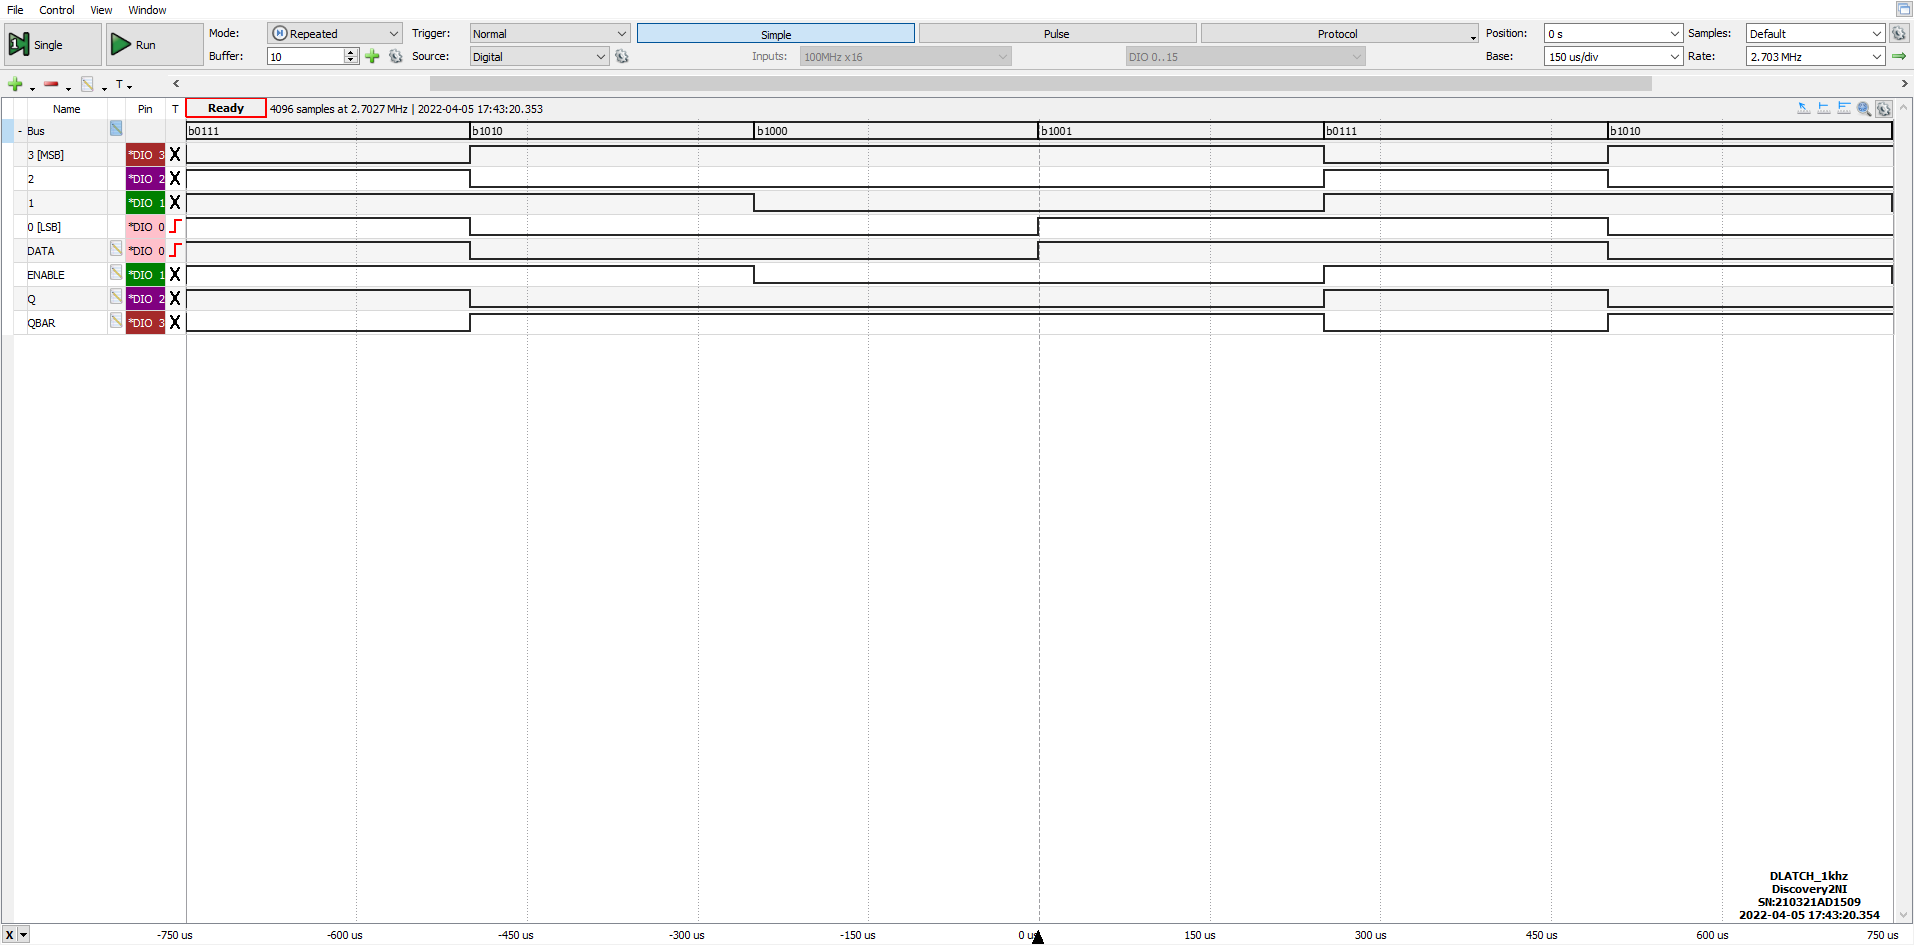
\includegraphics[width=\textwidth]{dlatch}
    \caption{Acquisizione di un ciclo completo (frequenza 1 kHz) con Logic
    Analyzer dei segnali in ingresso ($D =$ DIO 0, $E =$ DIO 1) e in uscita
    ($Q =$ DIO 2, $\overline{Q} =$ DIO 3) dal D-Latch.
    \label{fig: dlatch}}
\end{figure}
\begin{figure}[htbp]
	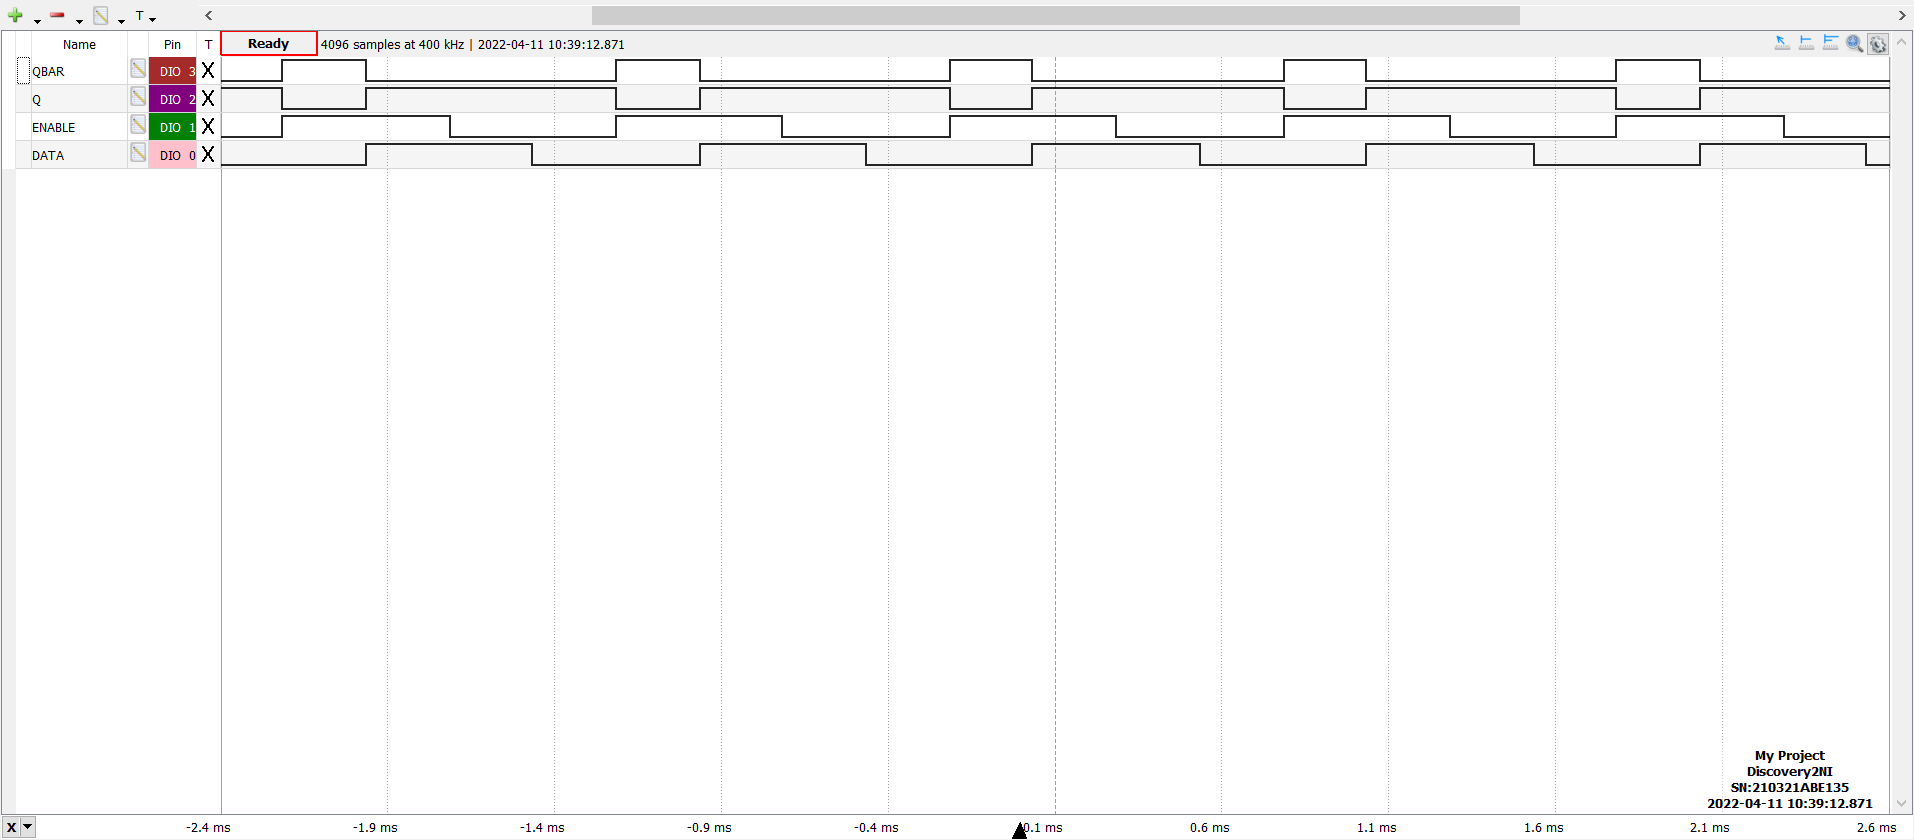
\includegraphics[width=\textwidth]{latch2}
	\caption{Acquisizione con Logic dell'andamento temporale dei segnali in
	ingresso uscita dal D-Latch per $\phi = -\SI{90}{\degree}$.
	\label{fig: Log_DLATCH2}}
\end{figure}

Dalle \cref{fig: dlatch} e \cref{fig: Log_DLATCH2} si osserva come durante lo
stato basso di Enable il segnale in uscita rimanga costante rispetto a
variazioni del segnale in $D$, mentre quando
$E = 1 \implies Q(t + \Delta t) = D$ coerentemente con quanto previsto dalla
tabella di verità e come principio di funzionamento della memoria a 1 bit.

\subsection{Misura dei tempi di propagazione nelle transizioni di stato}
Si riescono a distinguere due diverse transizioni dei segnali in ingresso per
ciascun valore di sfasamento tra i due segnali di clock in $D$ ed $E$;
per $\phi = \SI{90}{\degree}$:
\begin{enumerate}
\item $D \coloneqq 0$, $E: 0 \to 1$ \label{item: Efall}
\item $D: 0 \to 1$, $E \coloneqq 1$. \label{item: Drise}

Mentre per $\phi = - \SI{90}{\degree} = 270 \; \si{\degree}$:
\item $D: 1 \to 0$, $E \coloneqq 1$ \label{item: Dfall}
\item $D \coloneqq 1$, $E: 0 \to 1$. \label{item: Erise}
\end{enumerate}

Si sono misurati i ritardi tra la transizione dei segnali in ingresso e i
corrispondenti cambiamenti di stato in uscita su scala dei tempi minima
($\SI{10}{n\s}$) con i cursori dalle acquisizioni con Logic Analyzer e per
riconferma anche con l'oscilloscopio da banco (a cui associamo come
incertezza il contributo dato dalle specifiche del datasheet, tenendo conto
dell'instabilità e dello spessore delle tracce sullo schermo). Riportiamo
di seguito e nella \cref{fig: Drise}, \cref{fig: Drise_osc}, \cref{fig: Dfall}
e \cref{fig: Erise} i risultati ottenuti.
\begin{enumerate}
\item $t_{PHL} = 30 \pm 10 \; \si{n\s}$
\item $t_{PLH} = 20 \pm 10 \; \si{n\s}$

\item $t_{PHL} = 40 \pm 10 \; \si{n\s}$
\item $t_{PLH} = 30 \pm 10 \; \si{n\s}$
\end{enumerate}

\begin{figure}[htbp]
    \centering
    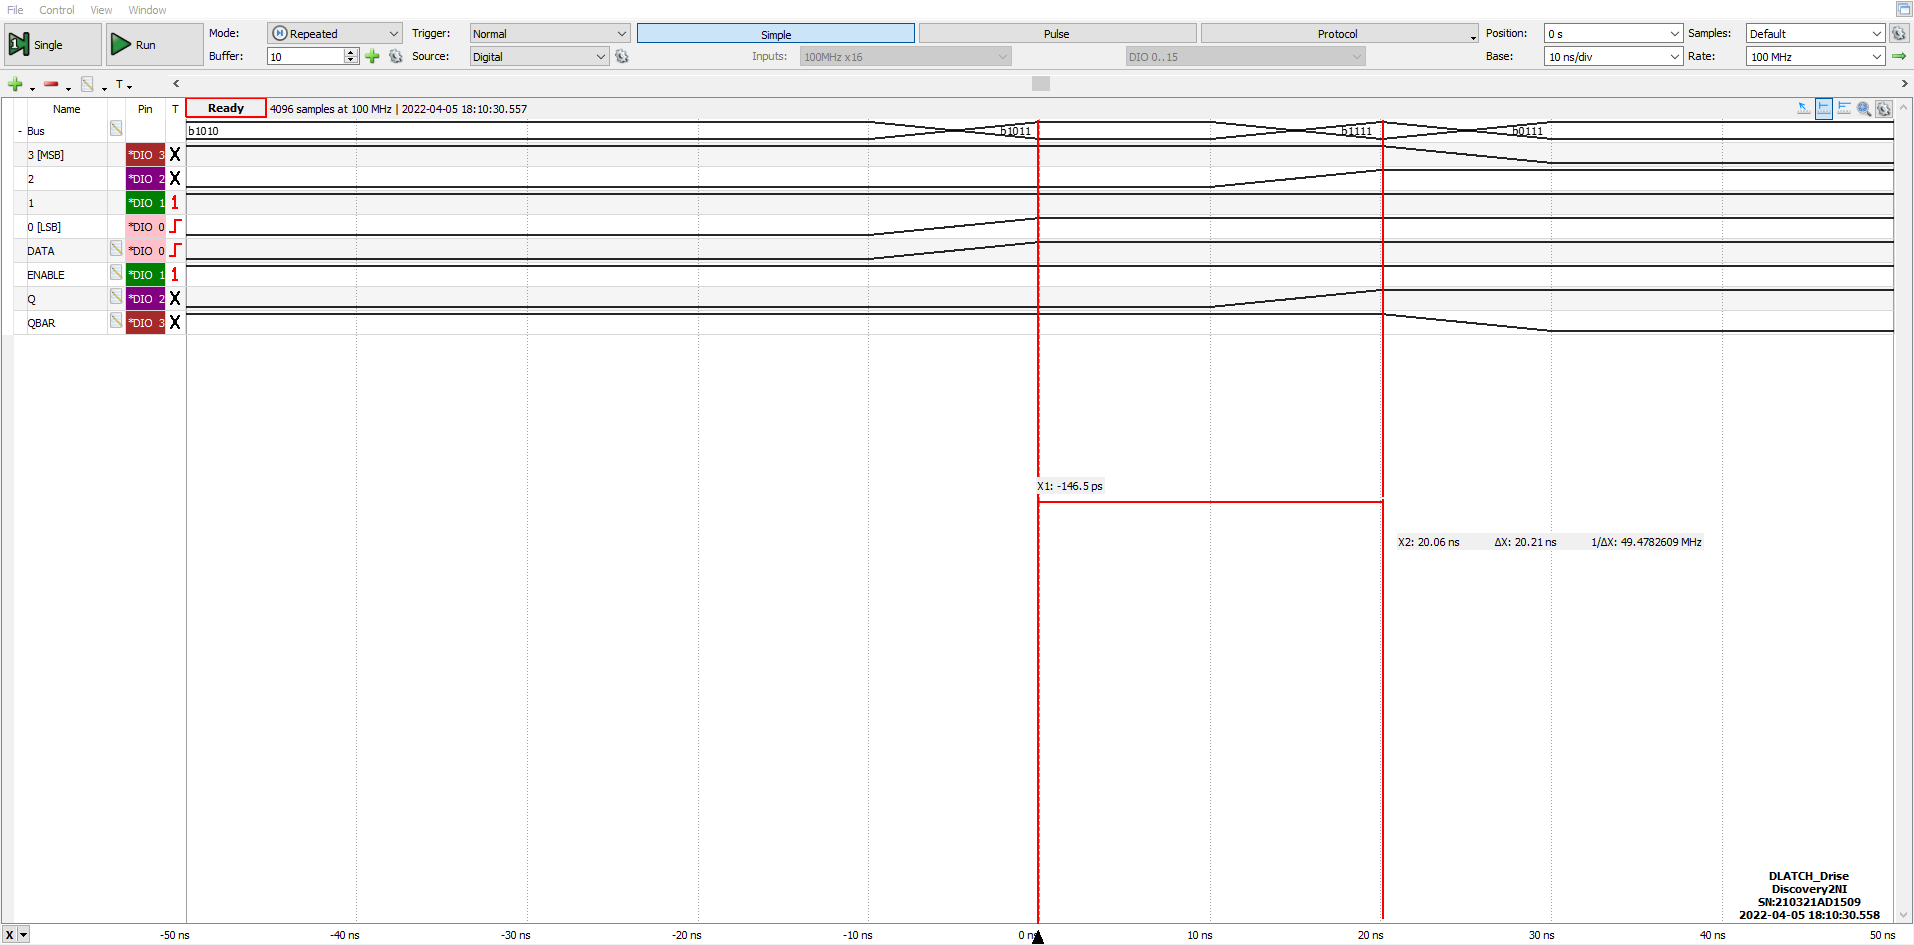
\includegraphics[width=\textwidth]{dlatch_Drise}
    \caption{Acquisizione del Logic Analyzer durante la transizione
    \ref{item: Drise} del D-Latch \label{fig: Drise}}
\end{figure}

\begin{figure}[htbp]
    \centering
    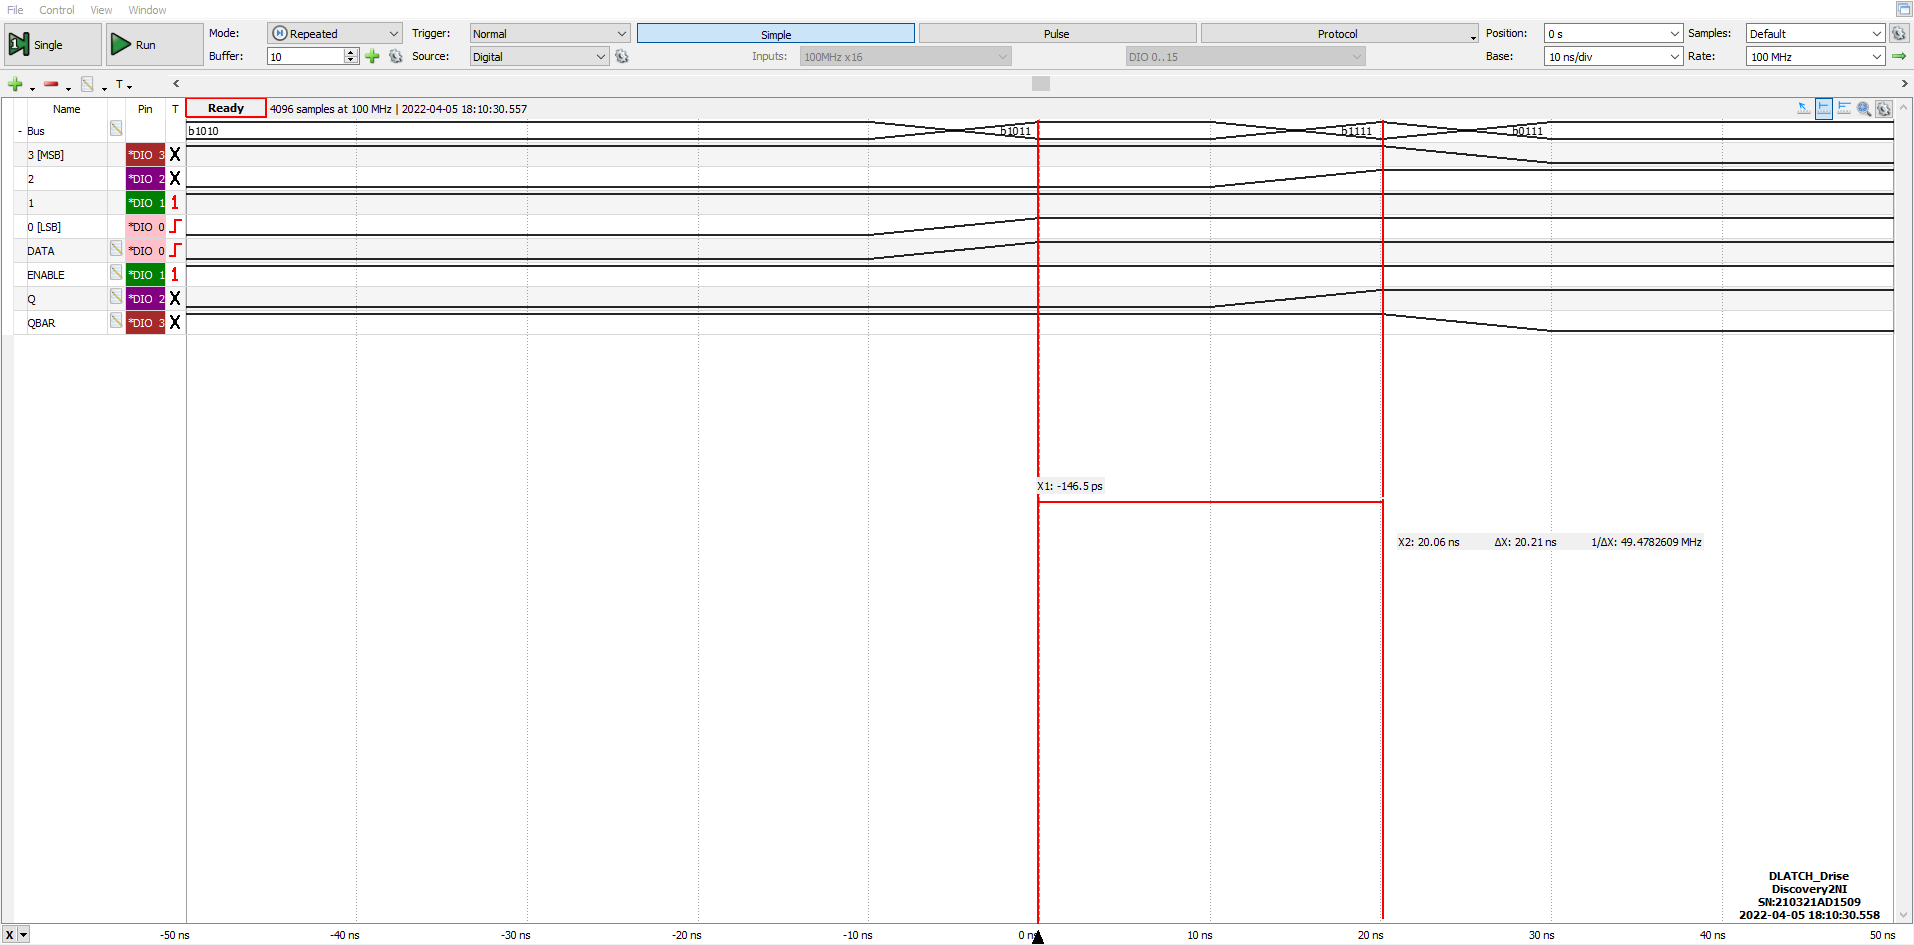
\includegraphics[width=\textwidth]{dlatch_Drise}
    \caption{Acquisizione da oscilloscopio digitale della transizione
    \ref{item: Drise} del D-Latch \label{fig: Drise_osc}}
    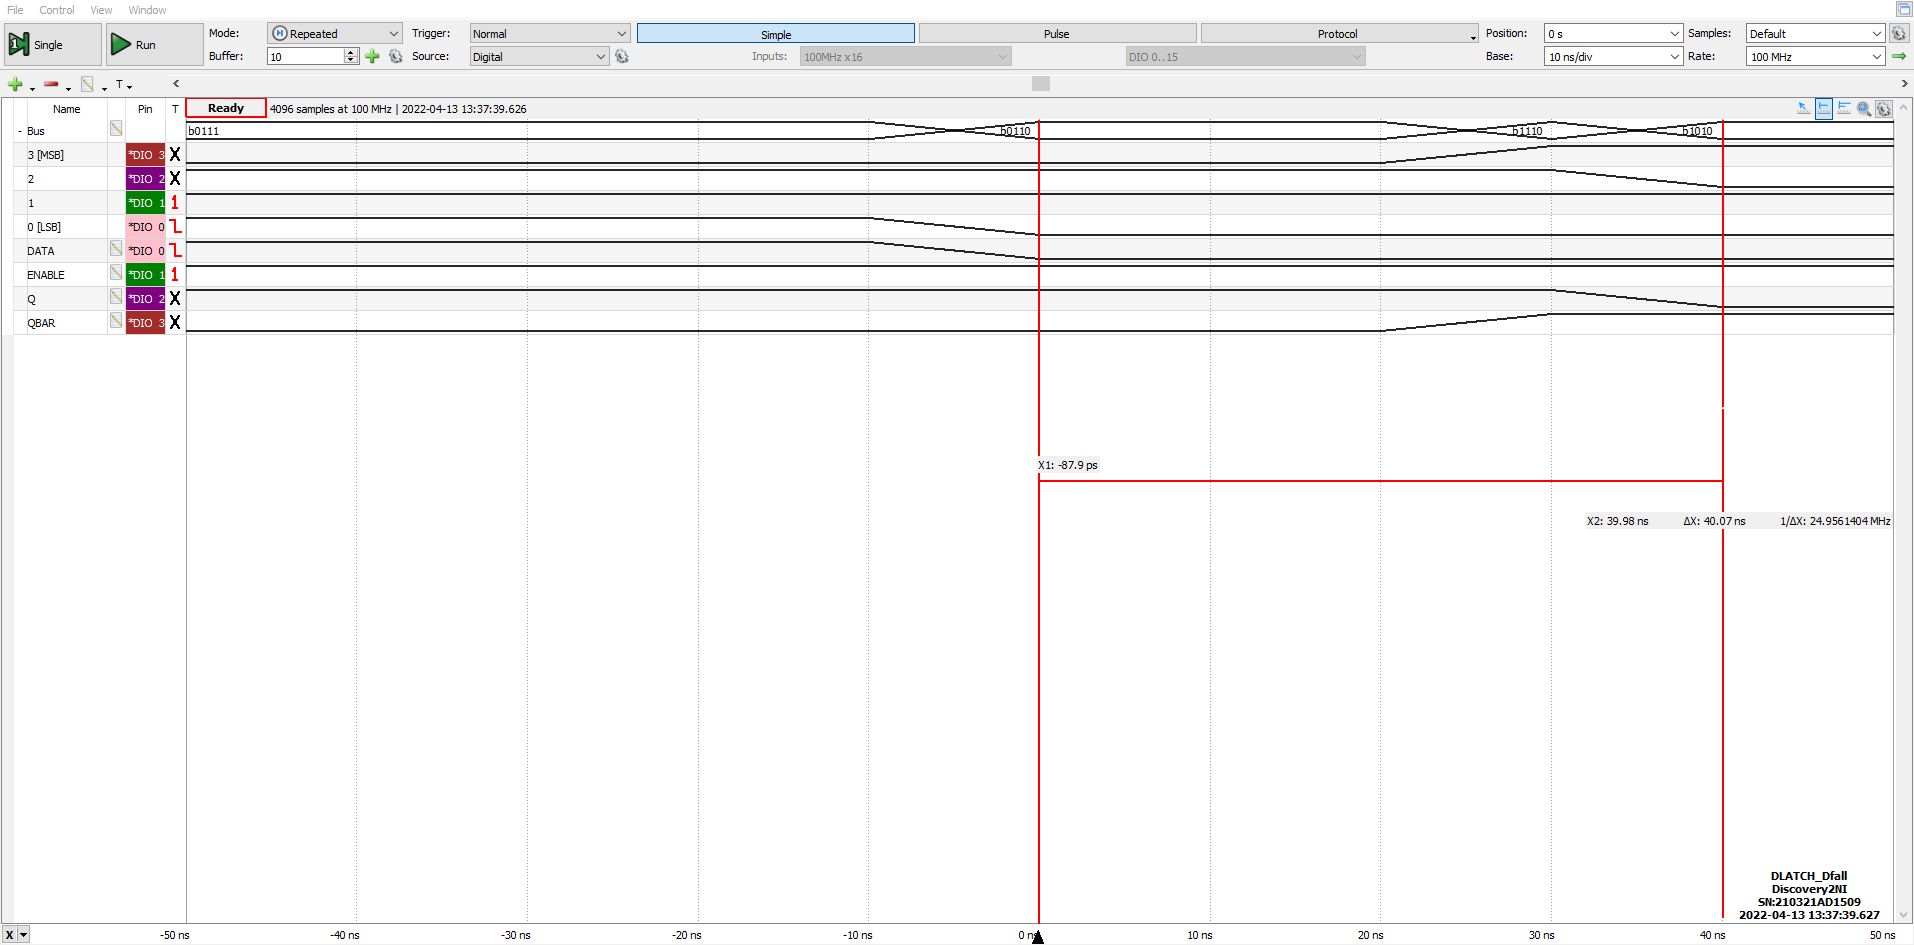
\includegraphics[width=\textwidth]{dlatch_Dfall40}
    \caption{Acquisizione del Logic Analyzer durante la transizione
    \ref{item: Dfall} del D-Latch \label{fig: Dfall}}
    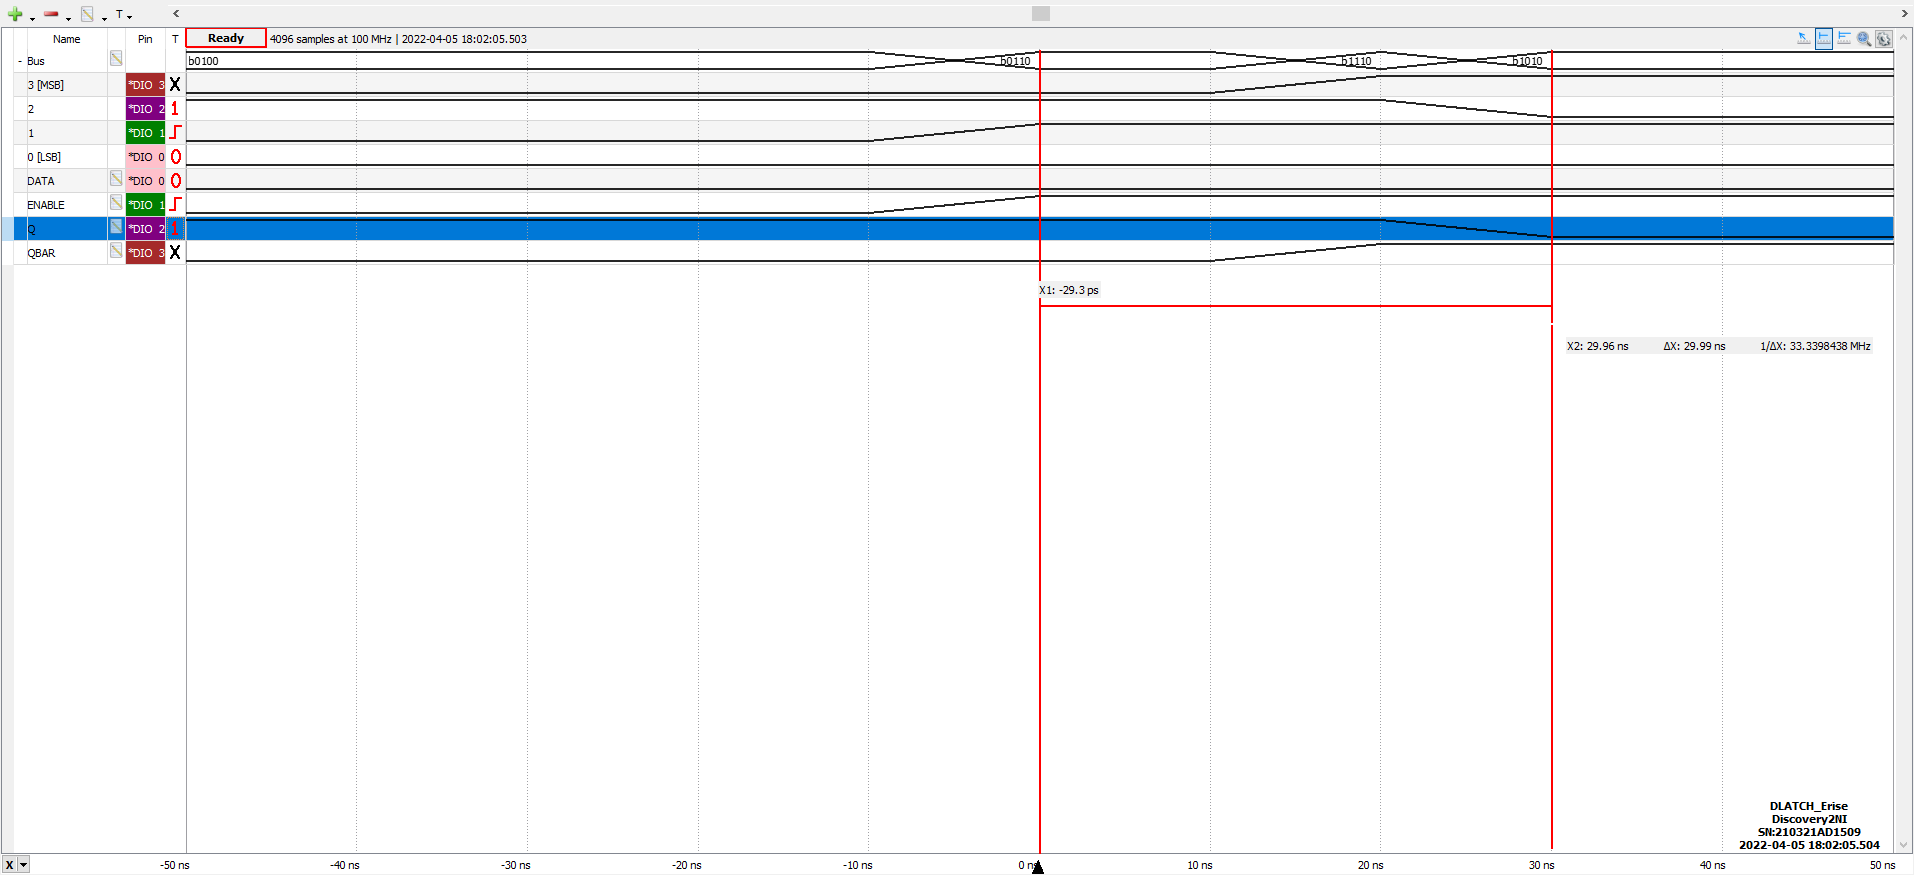
\includegraphics[width=\textwidth]{dlatch_Erise}
    \caption{Acquisizione del Logic Analyzer durante la transizione
    \ref{item: Erise} del D-Latch \label{fig: Erise}}
\end{figure}

Il massimo ritardo indotto si è trovato in corrispondenza della transizione
\ref{item: Dfall} dell'input $D$ da alto a basso (con i cursori
dell'oscilloscopio $t_{PHL} = 35 \pm 2 \; \si{n\s}$) mentre il minimo per la
\ref{item: Drise} (con oscilloscopio $t_{PLH} = 11 \pm 1 \; \si{n\s}$).

Dalle specifiche del DS si trova che i tempi di propagazione tipici e massimi
per una singola porta NAND sono:
\begin{table}[htbp]
\centering
\begin{tabular}{cccc}
	& typ & max & [units] \\
    $t\ped{PLH}$ & $11$ & $22$ & \si{n\s} \\
    $t\ped{PHL}$ & $7$ & $15$ & \si{n\s}
\end{tabular}
\end{table}
da cui vediamo che le nostre misure dei ritardi accumulati tra uscita e
ingresso del circuito sono compatibili con i tempi necessari per il numero di
porte NAND che devono commutare per il cambiamento di stato del D-Latch.

%=======================
\section{Shift-register con edge-triggered D-Flip Flop}
\subsection{Costruzione del circuito}
Si vuole ora costruire uno Shift Register a 4 bit a partire da due integrati
della serie SN74LS74 (Dual Positive-Edge-Triggered Flip-Flops), secondo lo
schema riportato in \cref{fig: schem_shift} e verificarne il funzionamento.
\begin{figure}[htbp]
\centering
	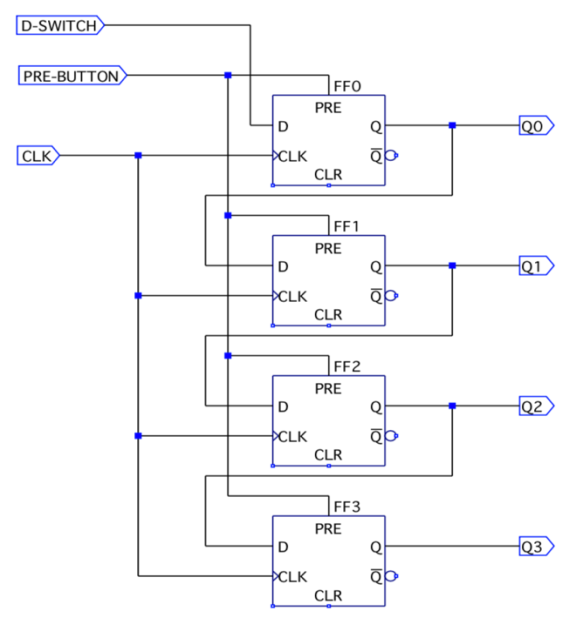
\includegraphics[width=0.6\textwidth]{schem_shift}
	\caption{\label{fig: schem_shift}}
\end{figure}

\subsection{Verifica della sincronia delle uscite rispetto a PRESET}
Una volta controllato che le uscite $Q_0$, $Q_1$, $Q_2$ e $Q_4$ fossero nello
stato $0000$, abbiamo utilizzato la funzione StaticIO per pilotare il PRESET
(ingresso PRE-BUTTON di \cref{fig: schem_shift}) tramite un pulsante inverso
(di tipo pressed$ = 0$ e released$ = 1$).
Dunque si è acquisito con Logic Analyzer l'andamento temporale dei 4 segnali
in uscita con condizione di trigger coincidente alla pressione del pulsante.
\begin{figure}[htbp]
\centering
	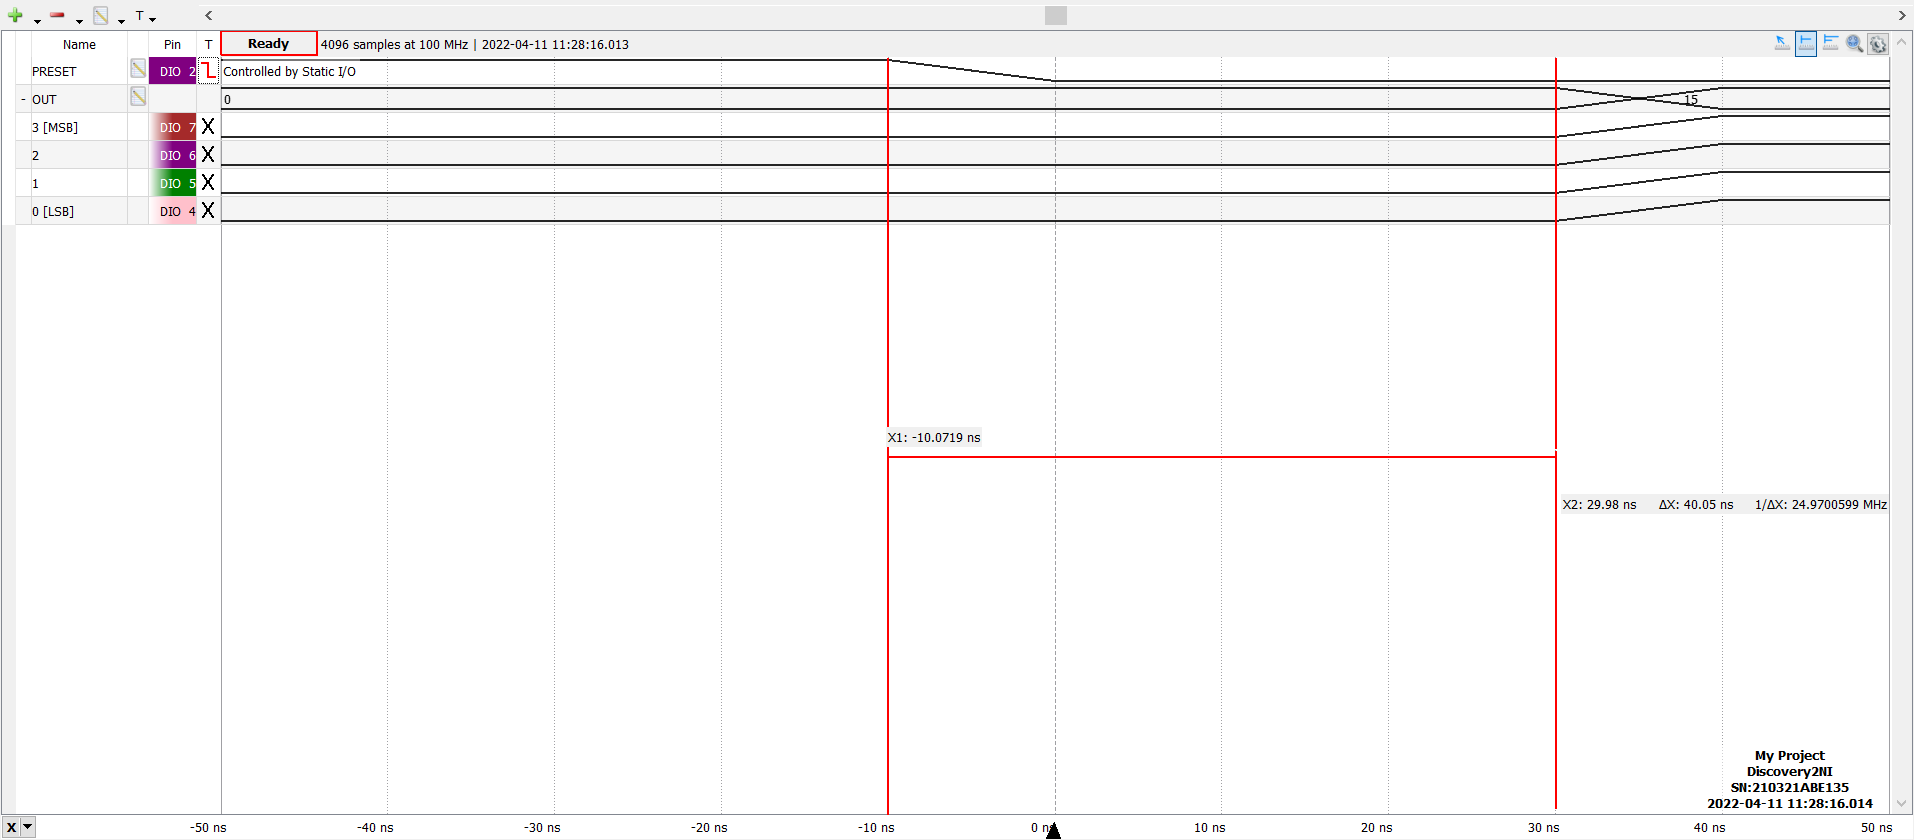
\includegraphics[width=\textwidth]{3.trans}
	\caption{Acquisizione con Logic dei segnali in PRE-BUTTON le 4 uscite dal
	registro a scorrimento pilotato dall'ingresso di PRESET
	\label{fig: Shift_reg_trans}}
\end{figure}

Dalla \cref{fig: Shift_reg_trans} vediamo che le commutazioni delle
uscite avvengono allo stesso tempo, dopo un $\Delta t = 40 \si{n\s}$ a partire
dalla pressione del pulsante di preset le 4 uscite raggiungono lo stato $1111$.

Nella \cref{fig: reg_presync} si mette in evidenza come questo cambiamento di
stato avvenga indipendentemente dal segnale di clock in ingresso ai FF, da cui
si vede che l'ingresso di PRESET dei Flip-Flop è asincrono come atteso dalle
specifiche tecniche.
\begin{figure}[htbp]
\centering
	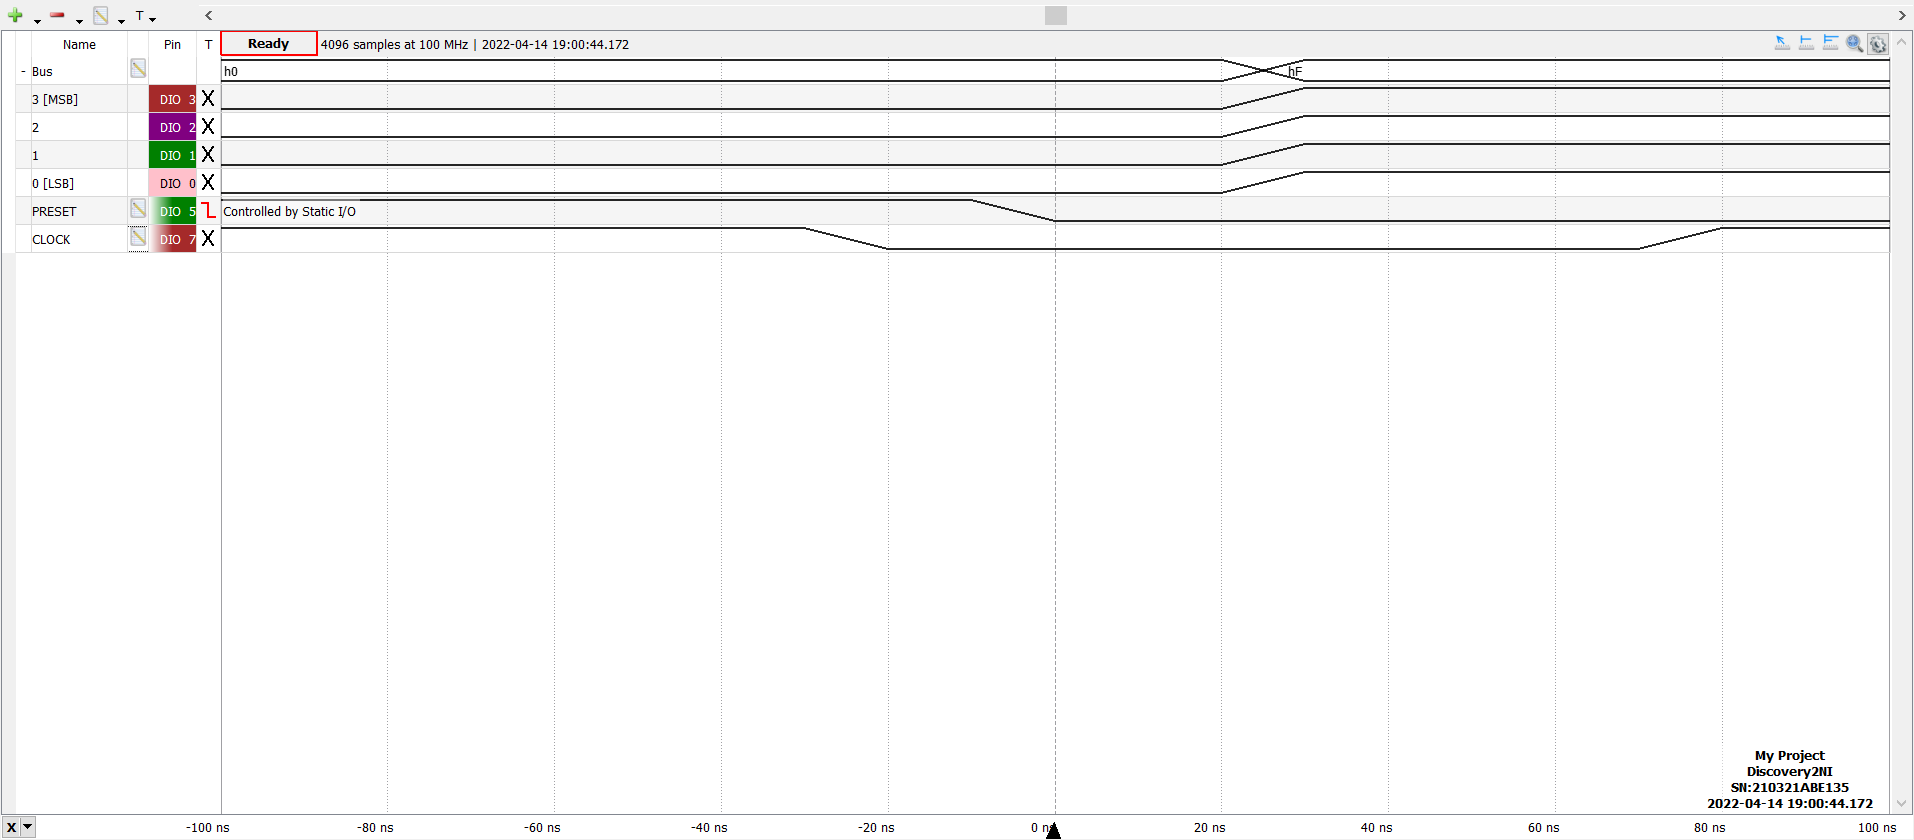
\includegraphics[width=\textwidth]{3.b}
	\caption{Acquisizione con Logic dei segnali in PRE-BUTTON, CLOCK e
	$Q_{0, \ldots, 3}$ in uscita dal registro a scorrimento studiato
	\label{fig: reg_presync}}
\end{figure}

\subsection{Verifica del funzionamento tramite clock}\label{sbs: clock_reg}
Possiamo costruire una tabella di verità per il registro in funzione del tempo
(discreto) battuto dal periodo $T$ del clock:
\begin{table}[htbp]
\centering
\begin{tabular}{c|c}
\toprule
$Q_i(t = t')$ & $Q_i(t = t' + T)$\\
\midrule
\midrule
$Q_0$ & $Q_0'$ \\
$Q_1$ & $Q_0(t=t')$ \\
$Q_2$ & $Q_1(t=t') = Q_0(t = t' - T)$ \\
$Q_3$ & $Q_2(t=t') = Q_0(t = t'- 2T)$ \\
\bottomrule
\end{tabular}
\caption{Tabella "di verità" di un registro a scorrimento, in cui $Q_0'$ è il
valore che viene inviato durante il fronte di salita $t'$ del clock tramite
il $D$-SWITCH
\label{tab: S-register}}
\end{table}

Nel caso in cui il pulsante di PRESET inizializzi tutte le uscite a 1, e il
D-Switch sia impostato (sempre con StaticIO) al valore $Q_0' = 0$, la
\cref{tab: S-register} si traduce nelle commutazioni di stato previste dalla
\cref{tab: s-reg-truth}
\begin{table}[htbp]
	\centering
	\begin{tabular}{c|cccc}
	\toprule
	$t$	  &		$Q_0$	&	$Q_1$	& $Q_2$	&	$Q_3$  \\
	\midrule
	\midrule
		$t'$ 	&	$1$	&	$1$	&	$1$	&	$1$	\\
		$+T$	&	$0$	&	$1$	&	$1$	&	$1$	\\
		$+2T$	&	$0$	&	$0$	&	$1$	&	$1$	\\
		$+3T$	&	$0$	&	$0$	&	$0$	&	$1$	\\
		$+4T$	&	$0$	&	$0$	&	$0$	&	$0$	\\		
	\bottomrule
	\end{tabular}
\caption{Sequenza di transizioni che si osservano a partire da quando viene
premuto il pulsante di PRESET ($t'$) lasciando a livello basso il $D$-SWITCH
del registro a scorrimento. \label{tab: s-reg-truth}}
\end{table}

Per verificare il corretto funzionamento del circuito si pilota il registro
con un segnale di clock di frequenza $f = \SI{1}{\Hz}$ e si fa ancora uso di
Logic per acquisire gli andamenti nel tempo dei valori assunti dalle uscite.
\begin{figure}[htbp]
\centering
	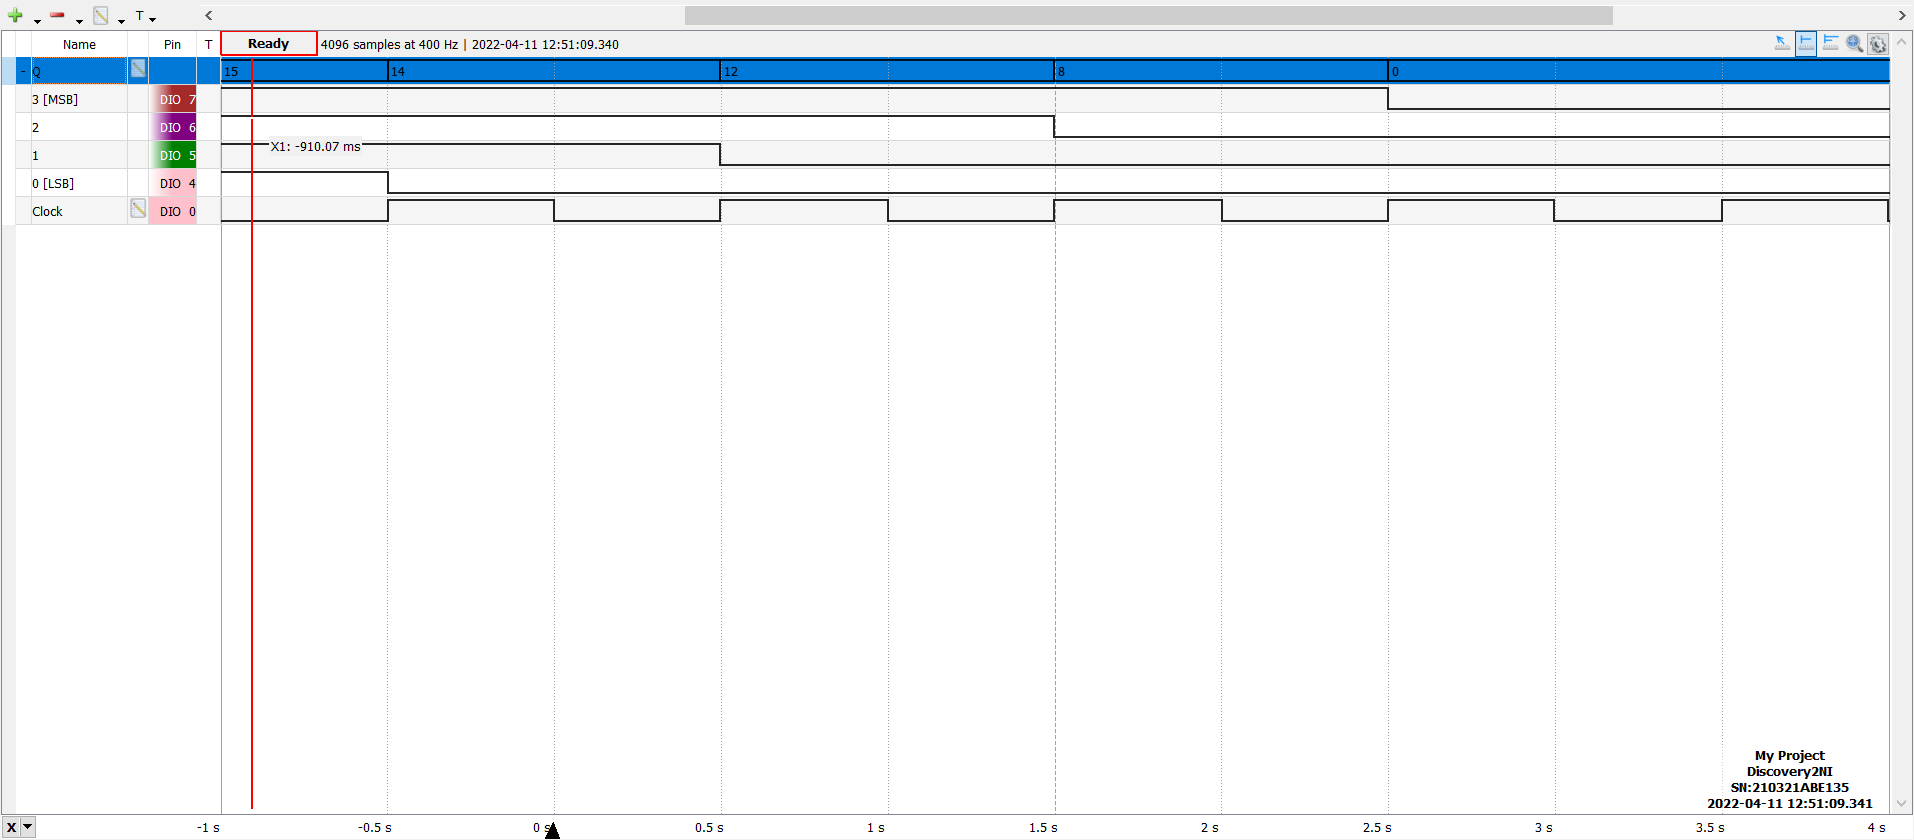
\includegraphics[width=\textwidth]{3.c}
	\caption{Acquisizione con Logic dei segnali in uscita da un registro a
	scorrimento di 4 bit come illustrato in \cref{sbs: clock_reg}
	\label{fig: Shift_reg_clock}}
\end{figure}
Dalla \cref{fig: Shift_reg_clock} si verifica come atteso che dopo 3 periodi
di clock (3 secondi) a partire da quando l'uscita $Q_0 = 0$, le 4 uscite
diventano (e si mantengono costanti nel tempo visto che il D-Switch rimane
fisso a 0) tutte quante basse.

Da questo si intuisce che collegando l'uscita (NOT) $Q_3$ all'ingresso
$D$-switch, possiamo generare una sequenza periodica/costruire un contatore
con modulo.

\subsection{Prevalenza tra gli ingressi D-switch e PRESET}
Utilizzando allo stesso tempo gli ingressi $D$-switch e PRESET del registro
si vede che è l'ultimo a pilotare il segnale in uscita, dal momento che PRESET
è asincrono (indipendente dalla salita del clock). Questo risulta consistente
con la regola generale per cui le architetture asincrone prendono la precedenza
sulle istruzioni sincrone. 

\subsection{Twisted-ring Johnson counter}
Dopo aver reimpostato il registro nello stato $Q_{i=0,\ldots, 3} = 0$, si
collega l'uscita $\overline{Q_3}$ all'ingresso $D$ del primo Flip-Flop e si
invia un clock di frequenza pari $f\ped{clk} = \SI{1}{k\Hz}$ all'ingresso del
circuito. Si riporta in \cref{fig: Shift_reg_seq} l'acquisizione con Logic
Analyzer dei segnali di clock e dei 4 output in funzione del tempo.
\begin{figure}[htbp]
\centering
	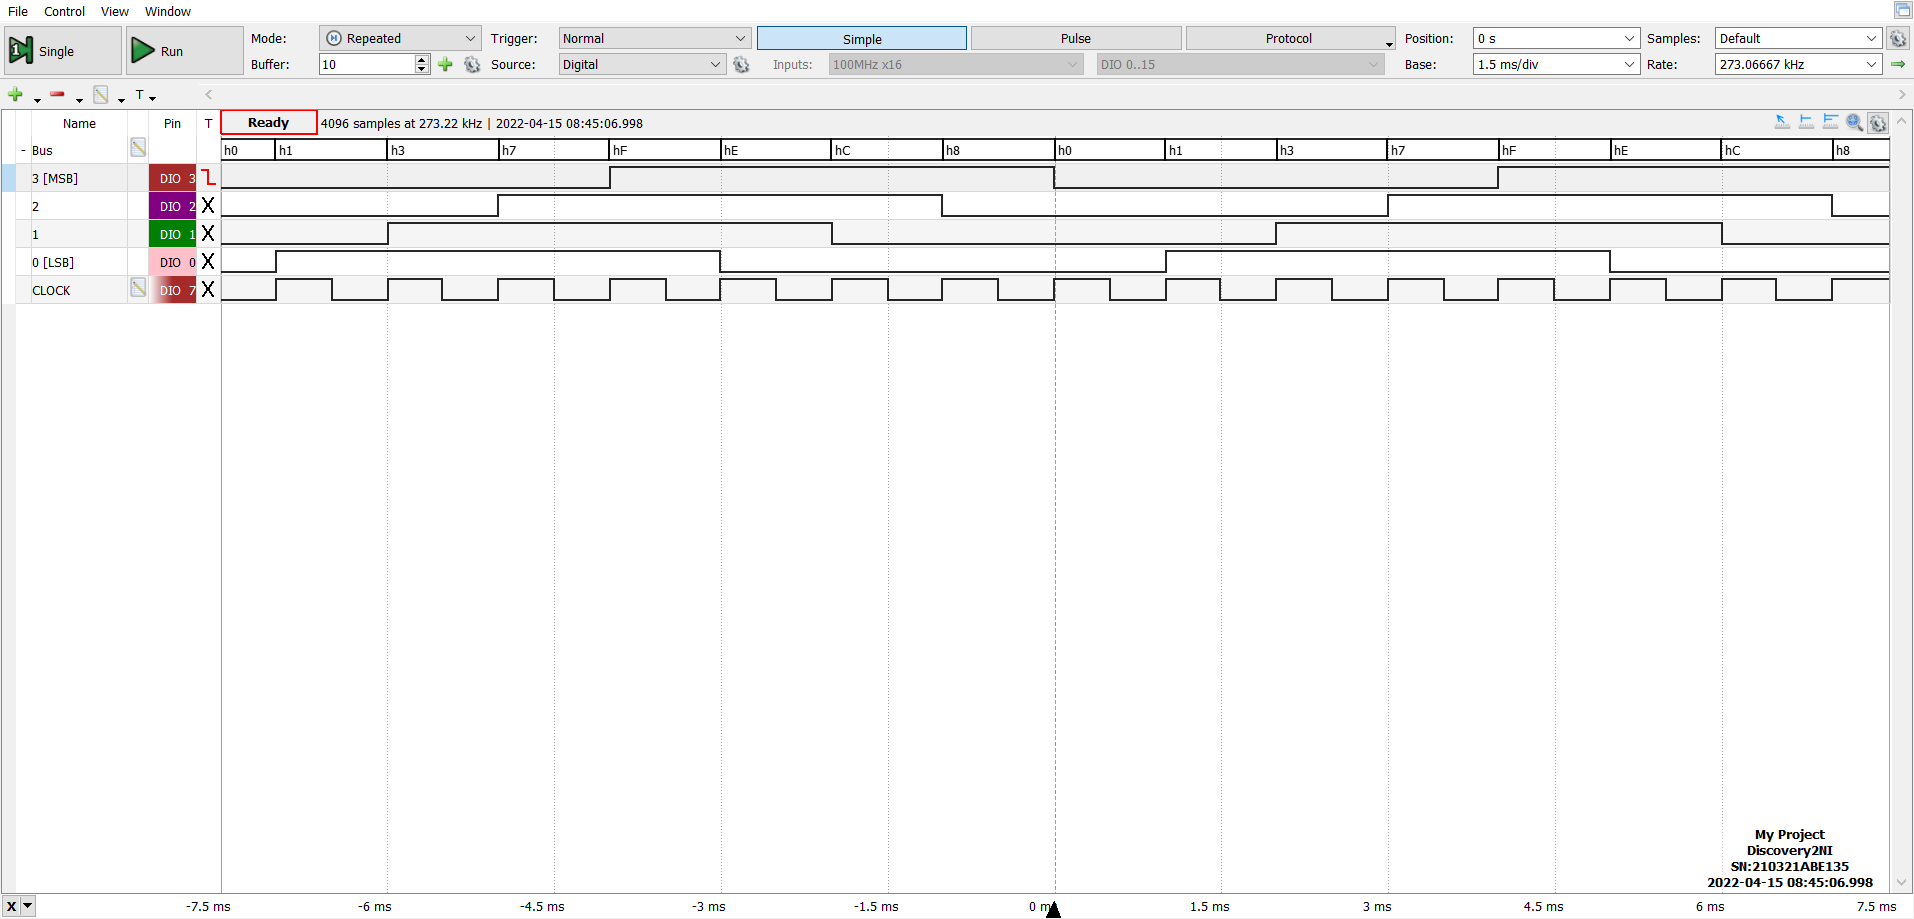
\includegraphics[width=\textwidth]{3.e}
	\caption{Acquisizione con Logic dei segnali in uscita dal registro a
	scorrimento con l'ultima uscita negata collegata all'ingresso del primo FF.
	\label{fig: Shift_reg_seq}}
\end{figure}

Da questa vediamo che in ogni uscita $Q_i$ si ha un'onda quadra con frequenza
$f = f\ped{clk}/8$, ciascuna traslata temporalmente di un periodo di clock
rispetto alla $Q_{i-1}$ precedente; per cui nel registro osserviamo la
sequenza atomica $00001111$ ripetersi ogni $8$ cicli di clock.

Questo è dovuto al fatto che nel registro ora scorre in modo ciclico la
concatenazione dello stato iniziale degli output e del suo negato (tramite
il collegamento ad anello $\overline{Q_3} \to Q_0$).
Supponendo infatti che nel circuito siano collegati ad anello $n$
edge-triggered Flip-Flop, in una qualsiasi delle uscite del twisted-ring
Johnson counter ci si aspetta di trovare un clock di frequenza divisa di un
fattore $2n$.

%=======================
\section{Generatore di sequenze pseudo-casuali}
\subsection{Costruzione del circuito}
Si vuole ora costruire un generatore di sequenze pseudo-casuali a 4 bit
utilizzando lo shift register studiato in precedenza e una porta XOR (dal chip
integrato SN74LS86 Quad XOR Gate).
La schematica del circuito che utilizzeremo è riportata in figura
\cref{fig: schem_gen}.
\begin{figure}[htbp]
\centering
	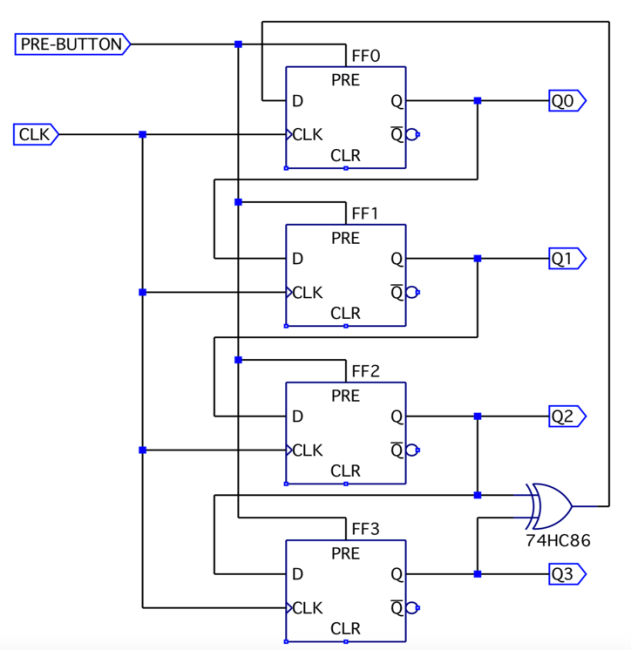
\includegraphics[width=0.6\textwidth]{schem_gen}
	\captionof{figure}{\label{fig: schem_gen}}
\end{figure}

\subsection{Analisi e verifica del funzionamento}
Dopo aver montato il circuito si inizializzano tutti Flip-Flop a 1 con
PRESET, si invia un segnale di clock a 10 kHz, sempre collegando gli output
$Q_{0,\ldots, 3}$ ai canali del Logic Analyzer per verificarne il
funzionamento.

Poiché il registro costruito ha memoria di $n = 4$ bit, dalla teoria ci
aspettiamo che la sequenza si ripeta dopo $2^4 = 16$ eventi al massimo,
condizione che si ottiene utilizzando come TAP (i.e. segnali in ingresso alla
porta XOR, la cui uscita è inviata all'ingresso $D = Q_0$ del primo FF) gli
output $Q_2$ (o $Q_0$) e $Q_3$.
\begin{figure}[htbp]
\centering
	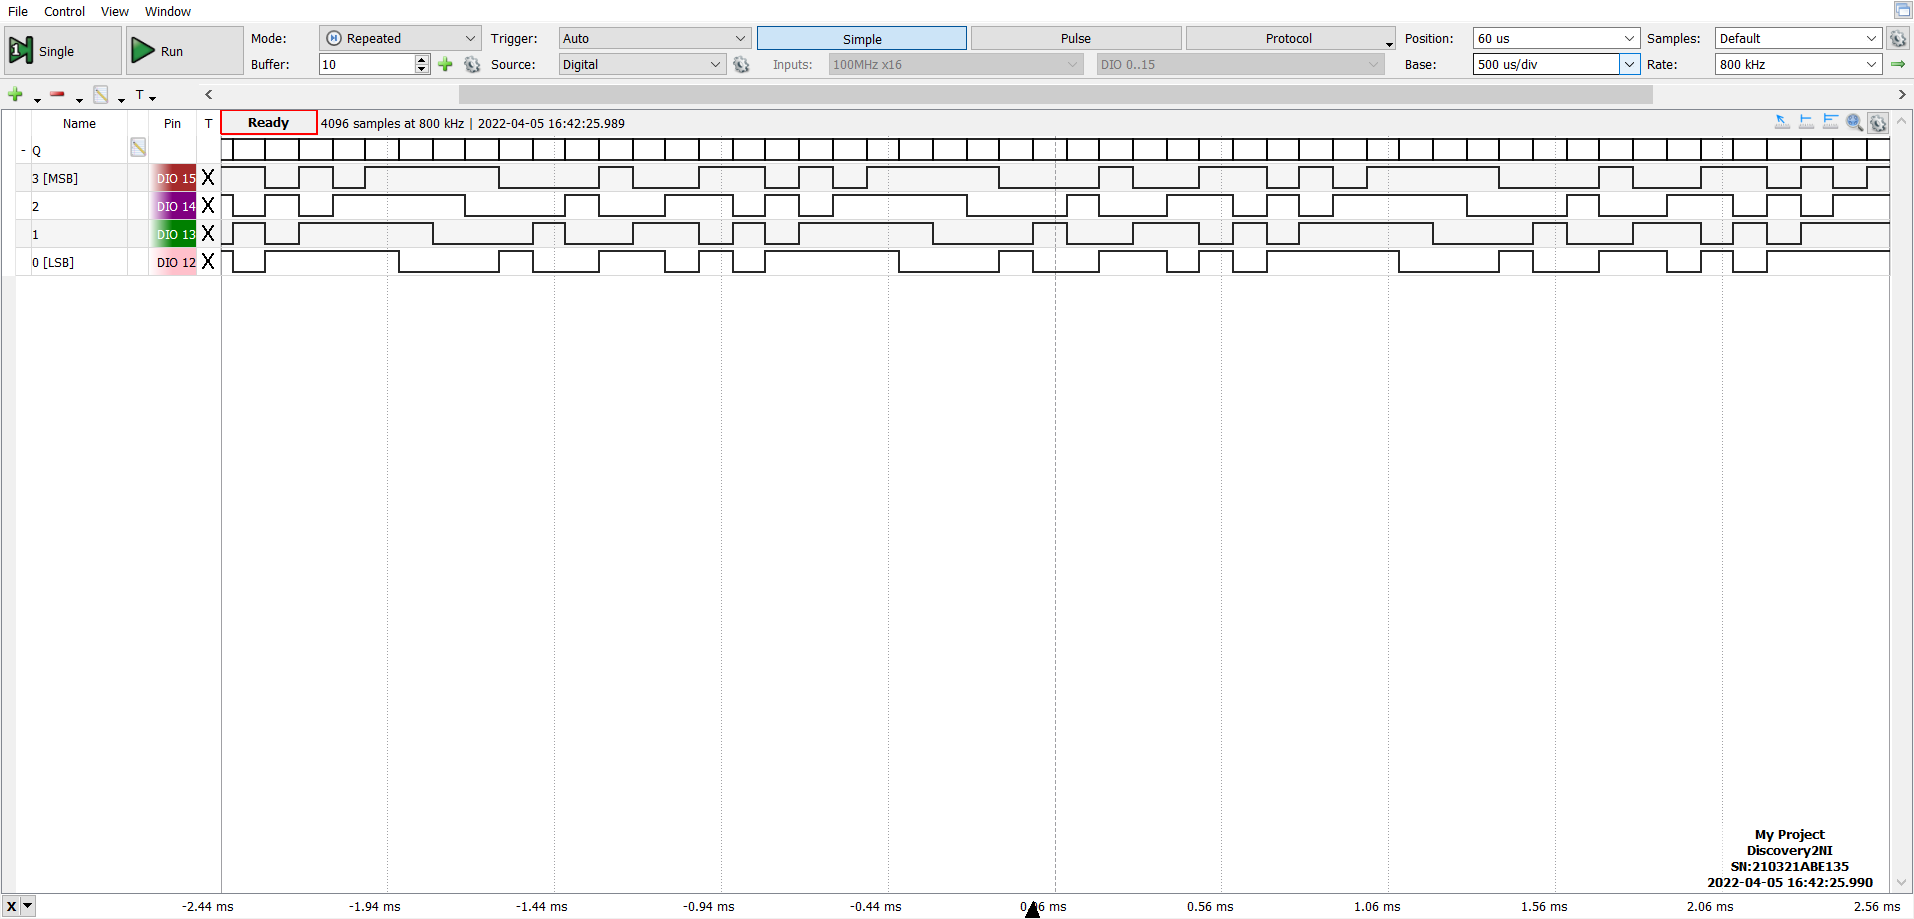
\includegraphics[width=\textwidth]{4.b}
	\caption{Acquisizione temporale con Logic del bus in uscita dal generatore
	di sequenze psudo-casuale descritto in \cref{fig: schem_gen}
	\label{fig: TAP_23}}
\end{figure}

\begin{table}[htbp]
\centering
\begin{tabular}{cccc}
\toprule
$Q_0$ & $Q_1$ & $Q_2$ & $Q_3$ \\
\midrule
\midrule
0 & 0 & 0 & 1 \\
0 & 0 & 1 & 0 \\
0 & 1 & 0 & 0 \\
1 & 0 & 0 & 1 \\
0 & 0 & 1 & 1 \\
0 & 1 & 1 & 0 \\
1 & 1 & 0 & 1 \\
1 & 0 & 1 & 0 \\
0 & 1 & 0 & 1 \\
1 & 0 & 1 & 1 \\
0 & 1 & 1 & 1 \\
1 & 1 & 1 & 1 \\
1 & 1 & 1 & 0 \\
1 & 1 & 0 & 0 \\
1 & 0 & 0 & 0 \\
\\
0 & 0 & 0 & 1 \\
\bottomrule
\end{tabular}
\caption{Sequenza pseudo-casuale attesa collegando come TAP alla porta XOR i
segnali $Q_2$ e $Q_3$ in uscita dal registro a scorrimento.
\label{tab: pseudo}}
\end{table}

Dall'acquisizione riportata in \cref{fig: TAP_23} si osserva la sequenza
riportata in \cref{tab: pseudo} ripetersi ogni 16 periodi di clock in accordo
con le aspettative (prendendo come riferimento una qualsiasi uscita dello
shift-register, visto che la sequenza nelle altre uscite sarà la medesima, ma
sfasata lungo l'asse temporale di qualche ciclo di clock).

\subsection{Studio delle sequenze generabili con diverse condizioni iniziali}
Si provano quindi altre combinazioni di TAP, per verificare che la scelta di
$Q_2$ e $Q_3$ produca una sequenza più lunga rispetto alle altre possibili
configurazioni. Riportiamo in \cref{fig: TAP_10}, \cref{fig: TAP_21} e
\cref{fig: TAP_30} i risultati ottenuti con Logic Analyzer dell'AD2.
\begin{figure}[htbp]
\centering
	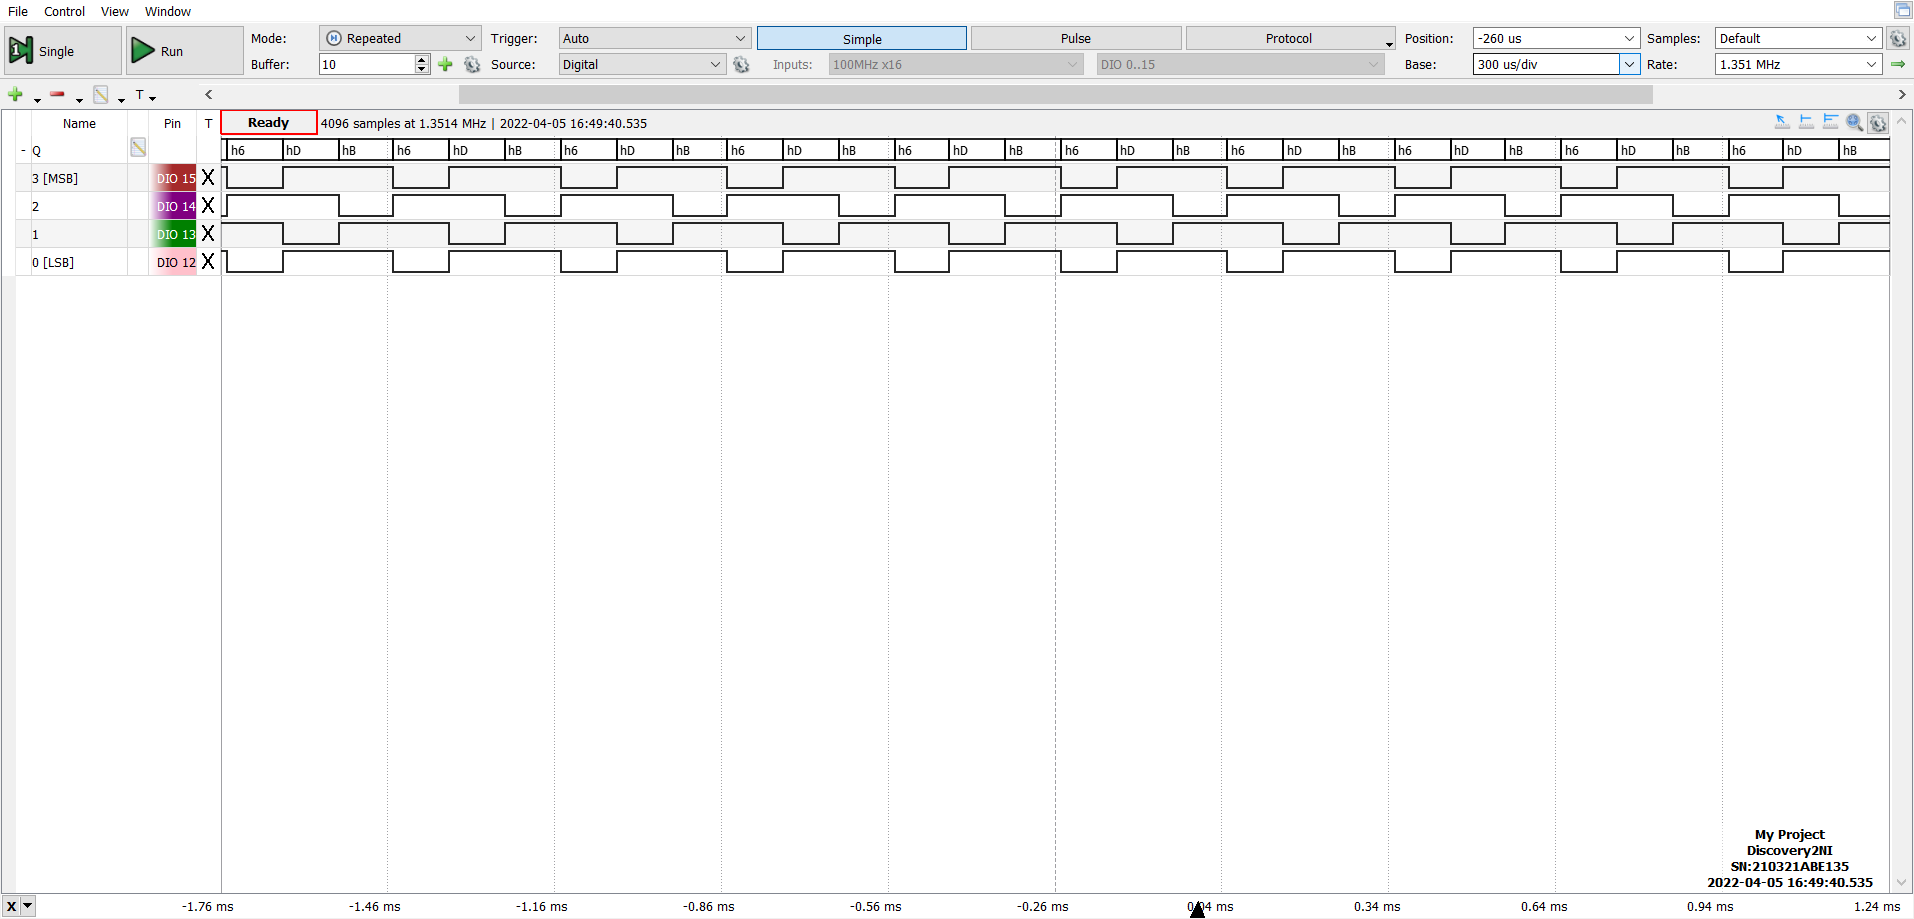
\includegraphics[width=\textwidth]{4.b_10}
	\caption{Acquisizione con Logic del bus in uscita dal generatore di sequenze
	pseudo-casuali con TAP sulle uscite $Q_0$ e $Q_1$; la sequenza si ripete ogni
	4 cicli di clock.
	\label{fig: TAP_10}}
\end{figure}
\begin{figure}[htbp]
\centering
	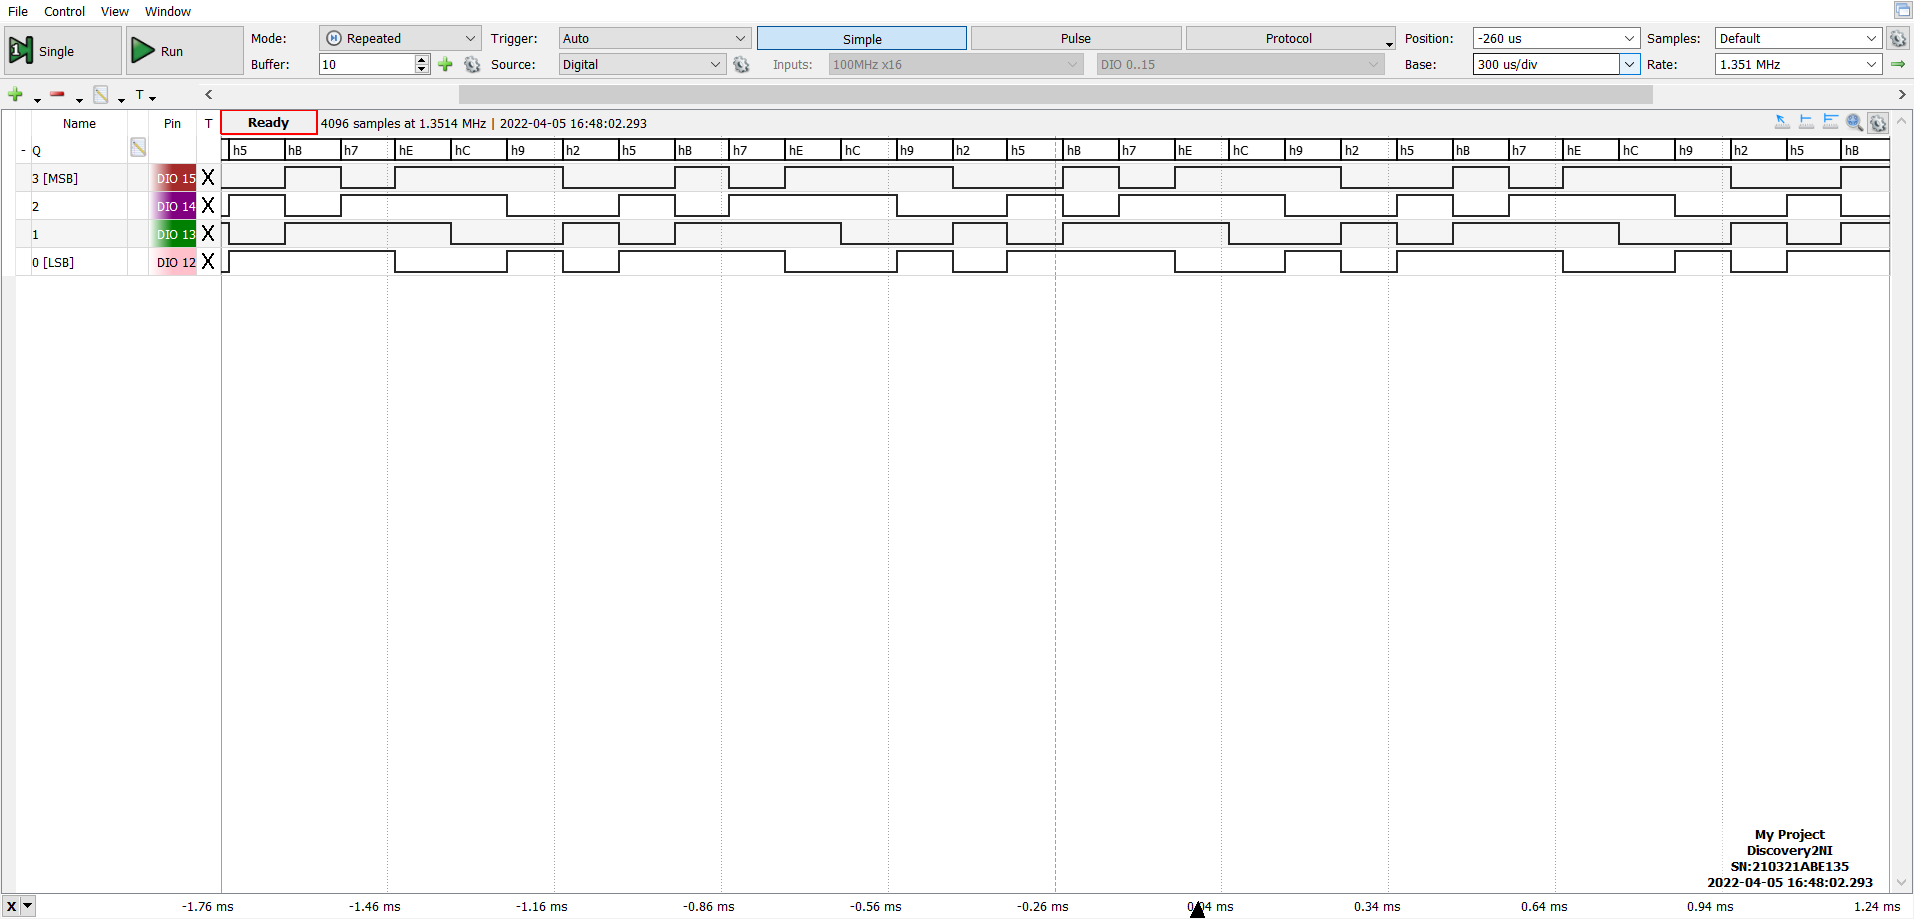
\includegraphics[width=\textwidth]{4.b_21}
	\caption{Acquisizione con Logic del bus in uscita dal generatore di sequenze
	pseudo-casuali con TAP sulle uscite $Q_2$ e $Q_1$; la sequenza si ripete ogni
	8 cicli di clock.
	\label{fig: TAP_21}}
\end{figure}
\begin{figure}[htbp]
\centering
	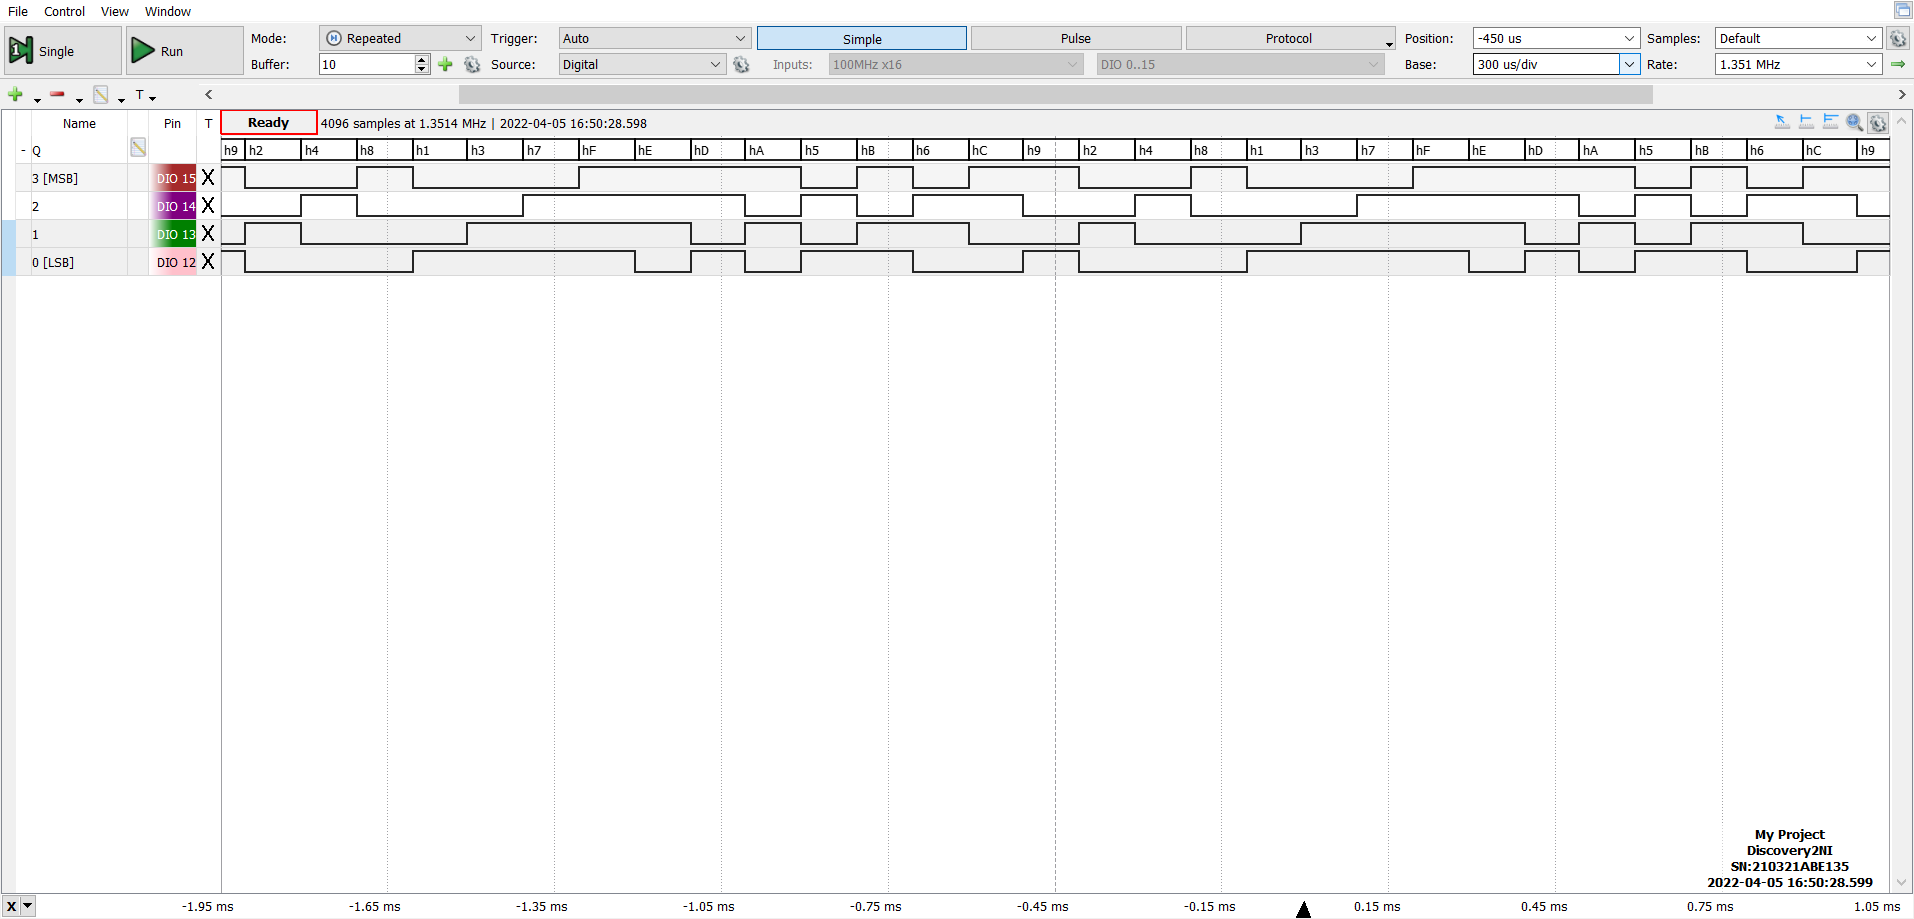
\includegraphics[width=\textwidth]{4.b_30}
	\caption{Acquisizione con Logic del bus in uscita dal generatore di sequenze
	pseudo-casuali con TAP sulle uscite La$Q_0$ e $Q_3$, la sequenza è massimale
	(si ripete ogni $2^n = 16$ cicli di clock).
	\label{fig: TAP_30}}
\end{figure}

%=======================
\section{Divisori di frequenza con contatori binari}
\subsection{Costruzione del circuito}
Si intende costruire un divisore di frequenza a partire da un contatore
binario a 4 bit (integrato SN74LS163 synchronous binary counter with
synchronous clear/load) secondo lo schema riportato in
\cref{fig: schem_counter}. 
\begin{figure}[htbp]
\centering
	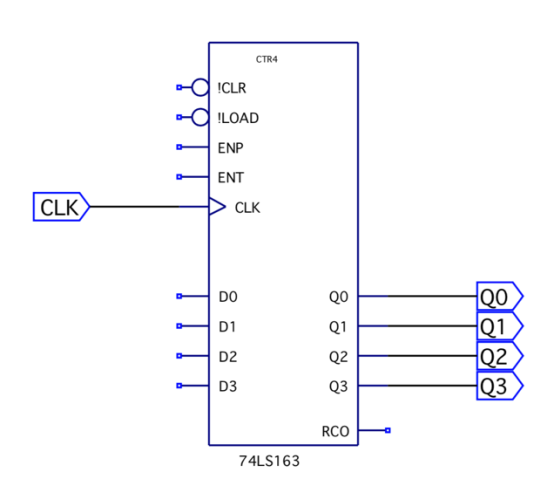
\includegraphics[width=0.6\textwidth]{schem_con}
	\caption{\label{fig: schem_counter}}
\end{figure}

\subsection{Verifica del ciclo di funzionamento dei contatori}
\label{sec: count_base}
Con la funzione Patterns di Waveform si invia un segnale di clock di
frequenza $f\ped{clk} = \SI{10}{k\Hz}$ al pin (CLK) del contatore e si
acquisiscono i segnali in uscita $Q_{0, \ldots, 3}$ con la funzione Logic
dello stesso.

Dalla \cref{fig: Count_Clock} si osserva che il bus ($Q_3 Q_2 Q_1 Q_0$ in
formato esadecimale) collegato ai segnali in uscita dal contatore a 4 bit
incrementa in maniera sequenziale dallo stato $0000$ (h0) fino allo stato
$1111$ (hF) in ordine crescente.
\begin{figure}[htbp]
\centering
	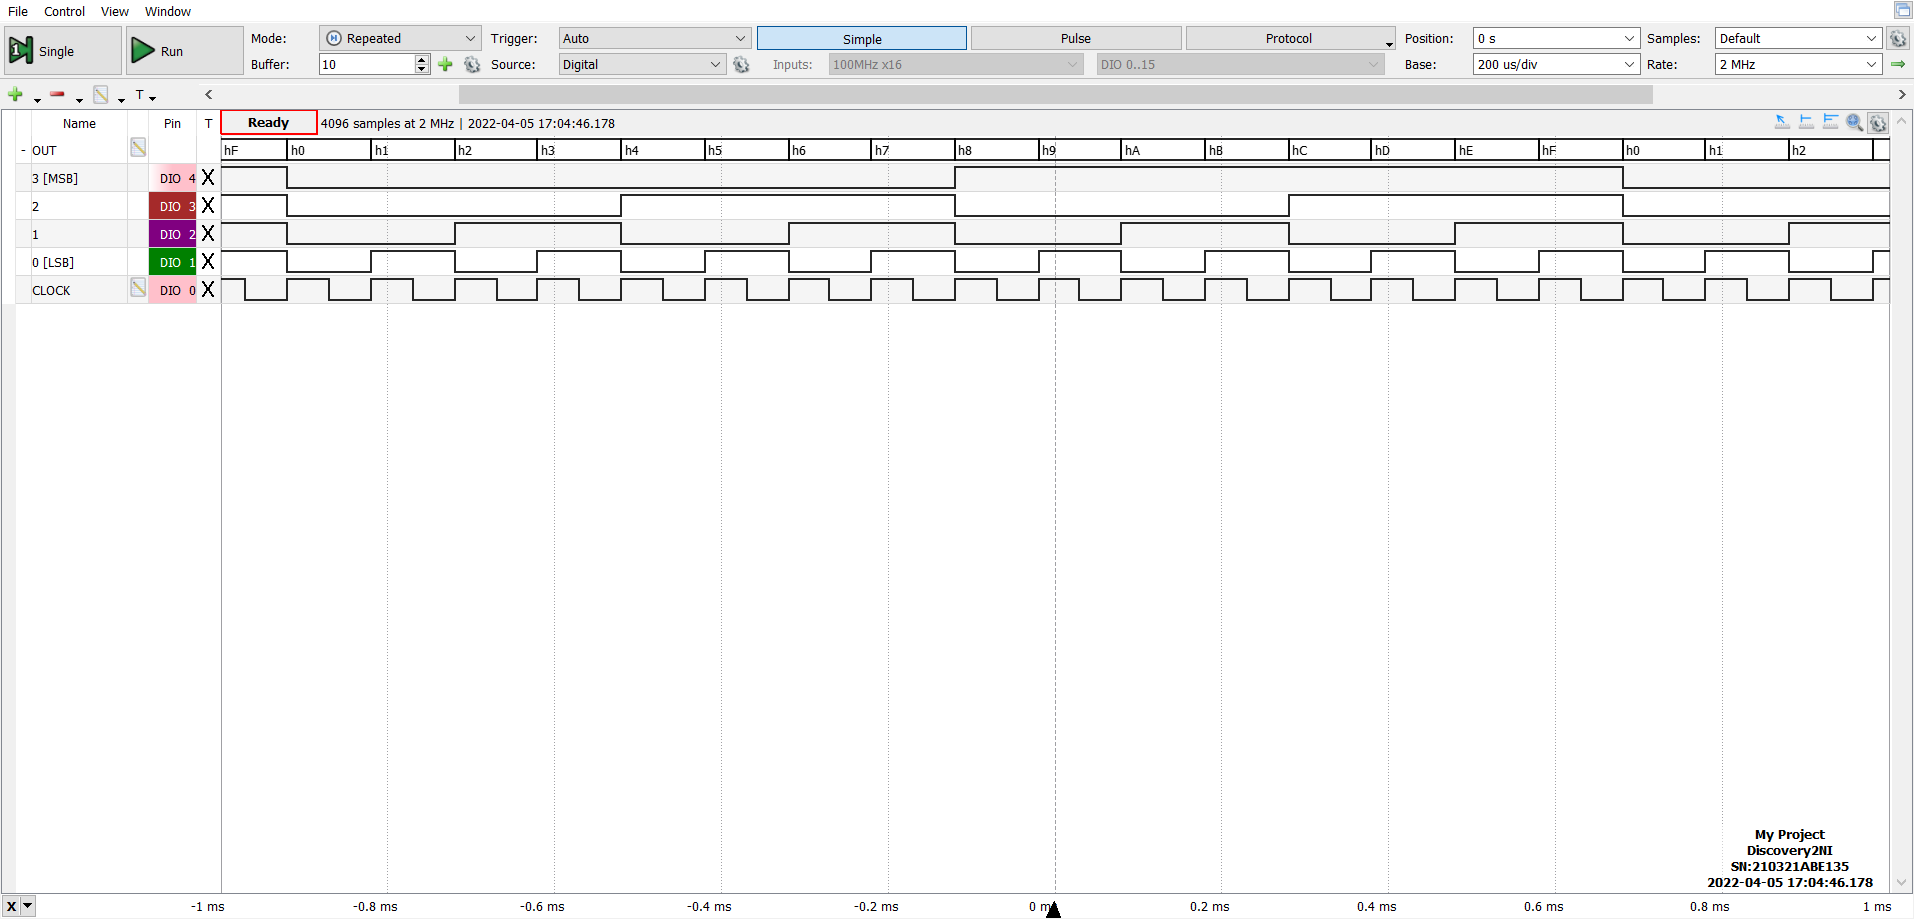
\includegraphics[width=\textwidth]{5.b}
	\caption{Acquisizione con Logic dell'andamento temporale dei segnali in
	uscita dal contatore SN74LS163, con frequenza di clock pari a 10 kHz.
	\label{fig: Count_Clock}}
\end{figure}

Da questa si verifica che il circuito esplora tutti gli stati possibili
nell'ordine corretto per il buon funzionamento del contatore a 4 bit.

\subsection{Verifica della divisione in frequenza}
Dato che il contatore (composto da 4 positive-edge-triggered FF) incrementa
di $1$ ad ogni fronte di salita del clock, ci si aspetta che il segnale di
ordine $i$ abbia come frequenza $f\ped{clk}/2^{i+1}$, la metà di quella del
bit precedente.

In termini del BUS di prima con parola di lunghezza 4 bit, ci si aspetta
quindi che le frequenze dei segnali per ciascun output del contatore siano:
\begin{itemize}
\item $\nicefrac{f\ped{clk}}{2}$ per il LSB $Q_0$
\item $\nicefrac{f\ped{clk}}{4}$ per $Q_1$
\item $\nicefrac{f\ped{clk}}{8}$ per $Q_2$
\item $\nicefrac{f\ped{clk}}{16}$ per il MSB $Q_3$
\end{itemize}
Sempre facendo riferimento alla \cref{fig: Count_Clock} risulta evidente come
le uscite del contatore si comportino da divisori in frequenza; infatti i
periodi che si trovano analizzando l'acquisizione sono rispettivamente 2 (LSB),
4, 8 e 16 (MSB) volte il periodo del clock $T\ped{clk} = 1/f\ped{clk}$.

\subsection{Transizione sincrona del contatore}
\label{sec: count_trans}
Impostiamo ora la condizione di trigger in Logic affinché l'acquisizione abbia
inizio quando il segnale in $Q_3$ scende da alto a basso, in modo da poter
studiare gli eventuali ritardi delle singole uscite nella transizione
$1111 \to 0000$ e verificare il comportamento sincrono del contatore.
\begin{figure}[htbp]
\centering
	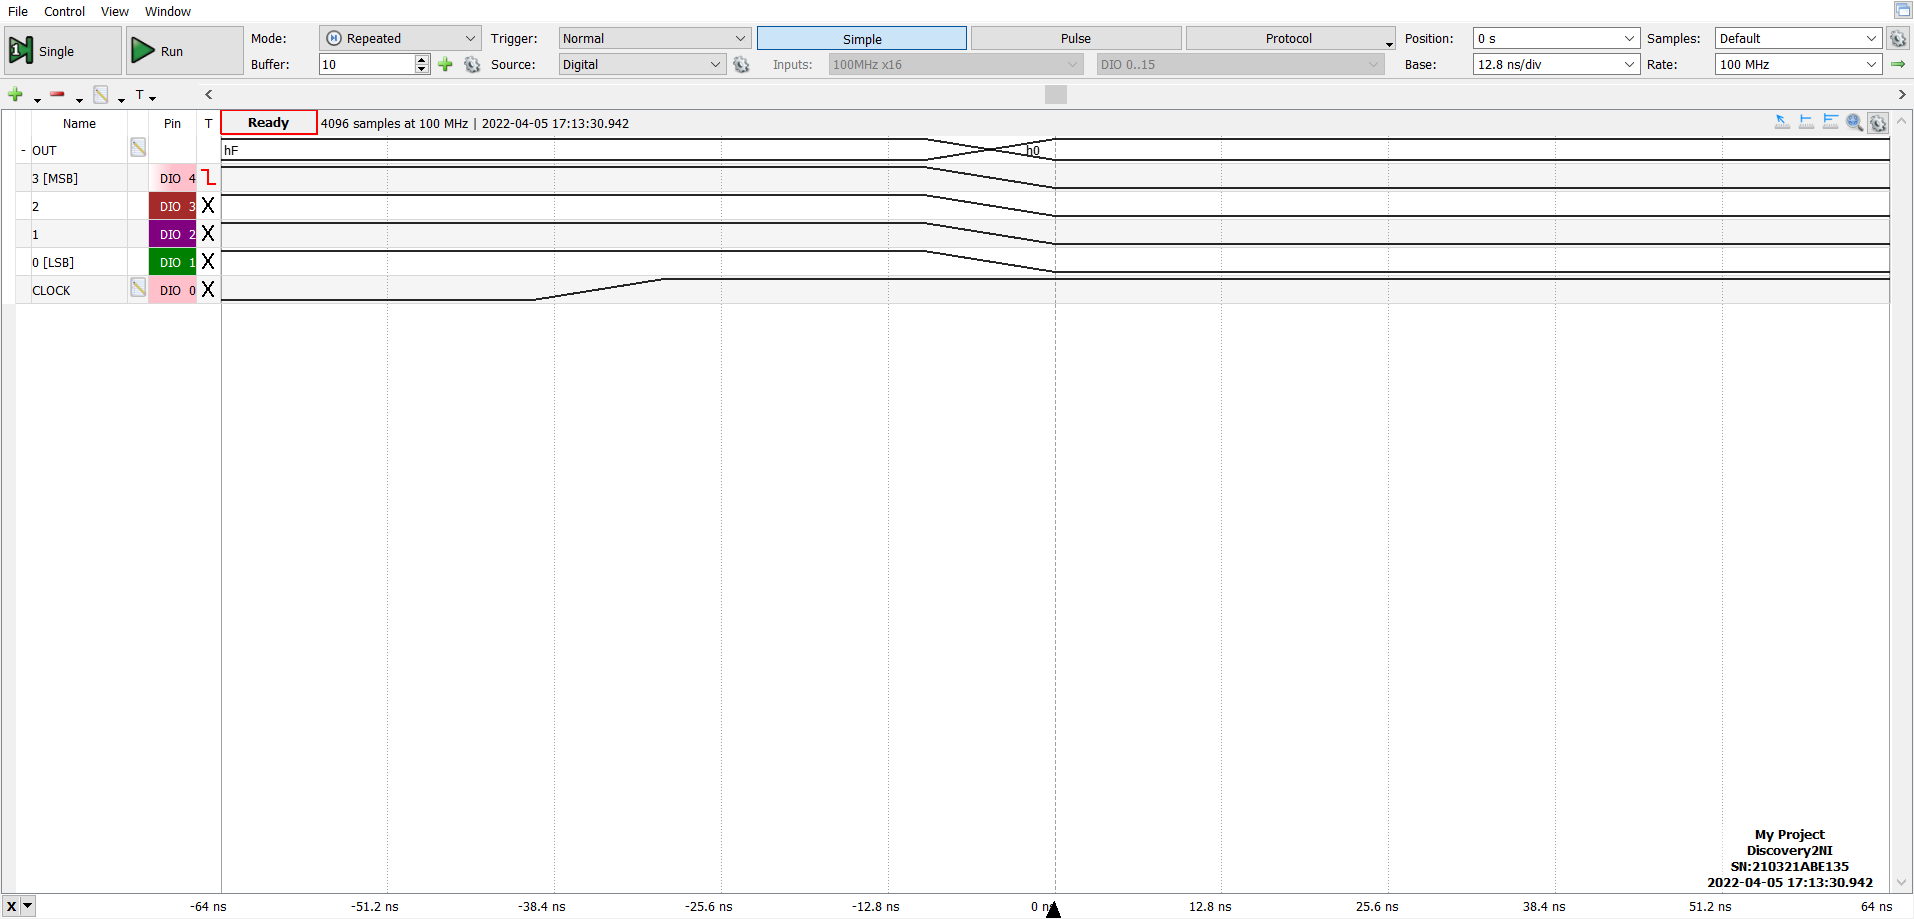
\includegraphics[width=\textwidth]{5.d}
	\caption{Acquisizione temporale con Logic del bus in uscita dal contatore durante la transizione 15->0; dall'immagine possiamo notare il comportamento sincrono della commutazione delle uscite del contatore \label{fig: Count_150}}
\end{figure}

Dalla \cref{fig: Count_150} possiamo vedere che la commutazione delle uscite è
sincrona e avviene simultaneamente per ogni pin di output con un ritardo di
$t_{PHL} = 30 \pm \; \si{n\s}$ dal fronte di salita del clock, in linea con
quanto previsto dalle specifiche dell'integrato.

\subsection{Divisore di frequenza 1/10; Contatore BCD}
Per realizzare un divisore in frequenza che generi un segnale di periodo pari
a $T = 10 T\ped{clk}$ facciamo uso del pin CLEAR (Active-Low) del contatore,
il quale resetta il contatore allo stato $0000$ quando riceve un segnale a
livello logico basso.
\begin{figure}[htbp]
\centering
	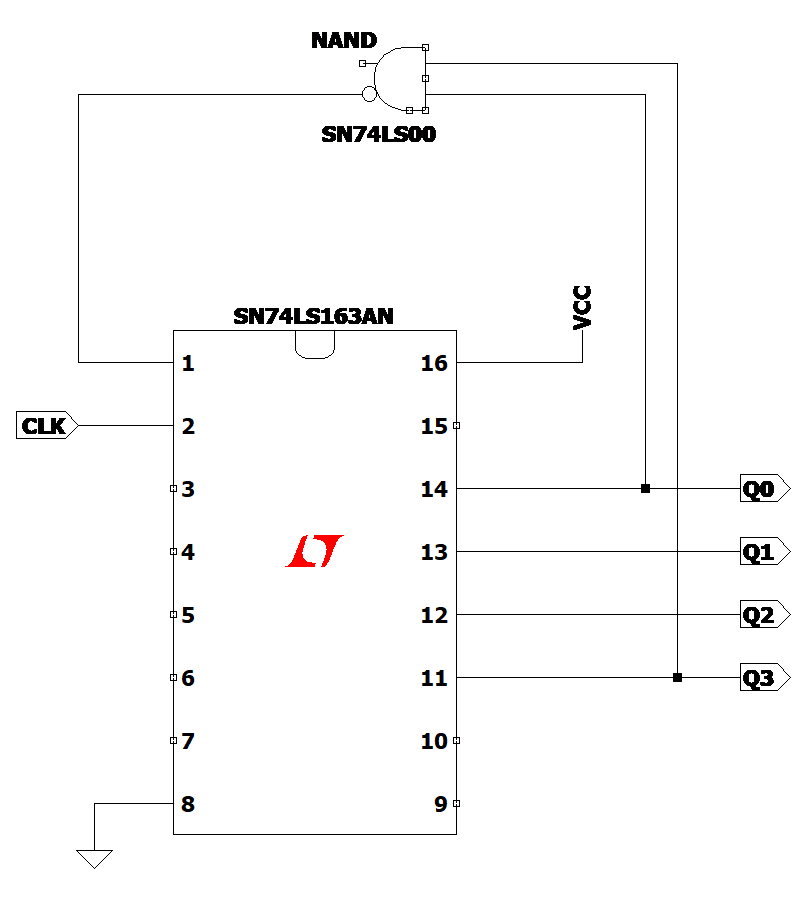
\includegraphics[width=0.6\textwidth]{Draft1}
	\caption{Schematica utilizzata per il divisore per 10 di frequenza
	\label{schem: 10_div}}
\end{figure}

Affinché il contatore raggiunga un totale di 10 stati prima di ripartire,
dobbiamo imporre la condizione che arrivati allo stato $9$ (b1001) il
contatore riceva il comando di reset da CLEAR.
Per farlo colleghiamo ai 2 ingressi di una porta NAND il LSB e il MSB e
la sua uscita al pin di Clear, cosicché quando il contatore arriva a 9
(entrambi $Q_0$ e $Q_3$ sono alti) CLEAR riceverà un segnale di reset,
per cui la frequenza del segnale in uscita da $Q_3$ corrisponderà ad un decimo
di quella di clock. Si riporta in \cref{schem: 10_div} lo schema proposto per
il circuito.

Come prima, si utilizza la funzione Logic per acquisire i segnali provenienti
dal Bus dei 4 bit in uscita, il clock e il bit di Clear.
\begin{figure}[htbp]
\centering
	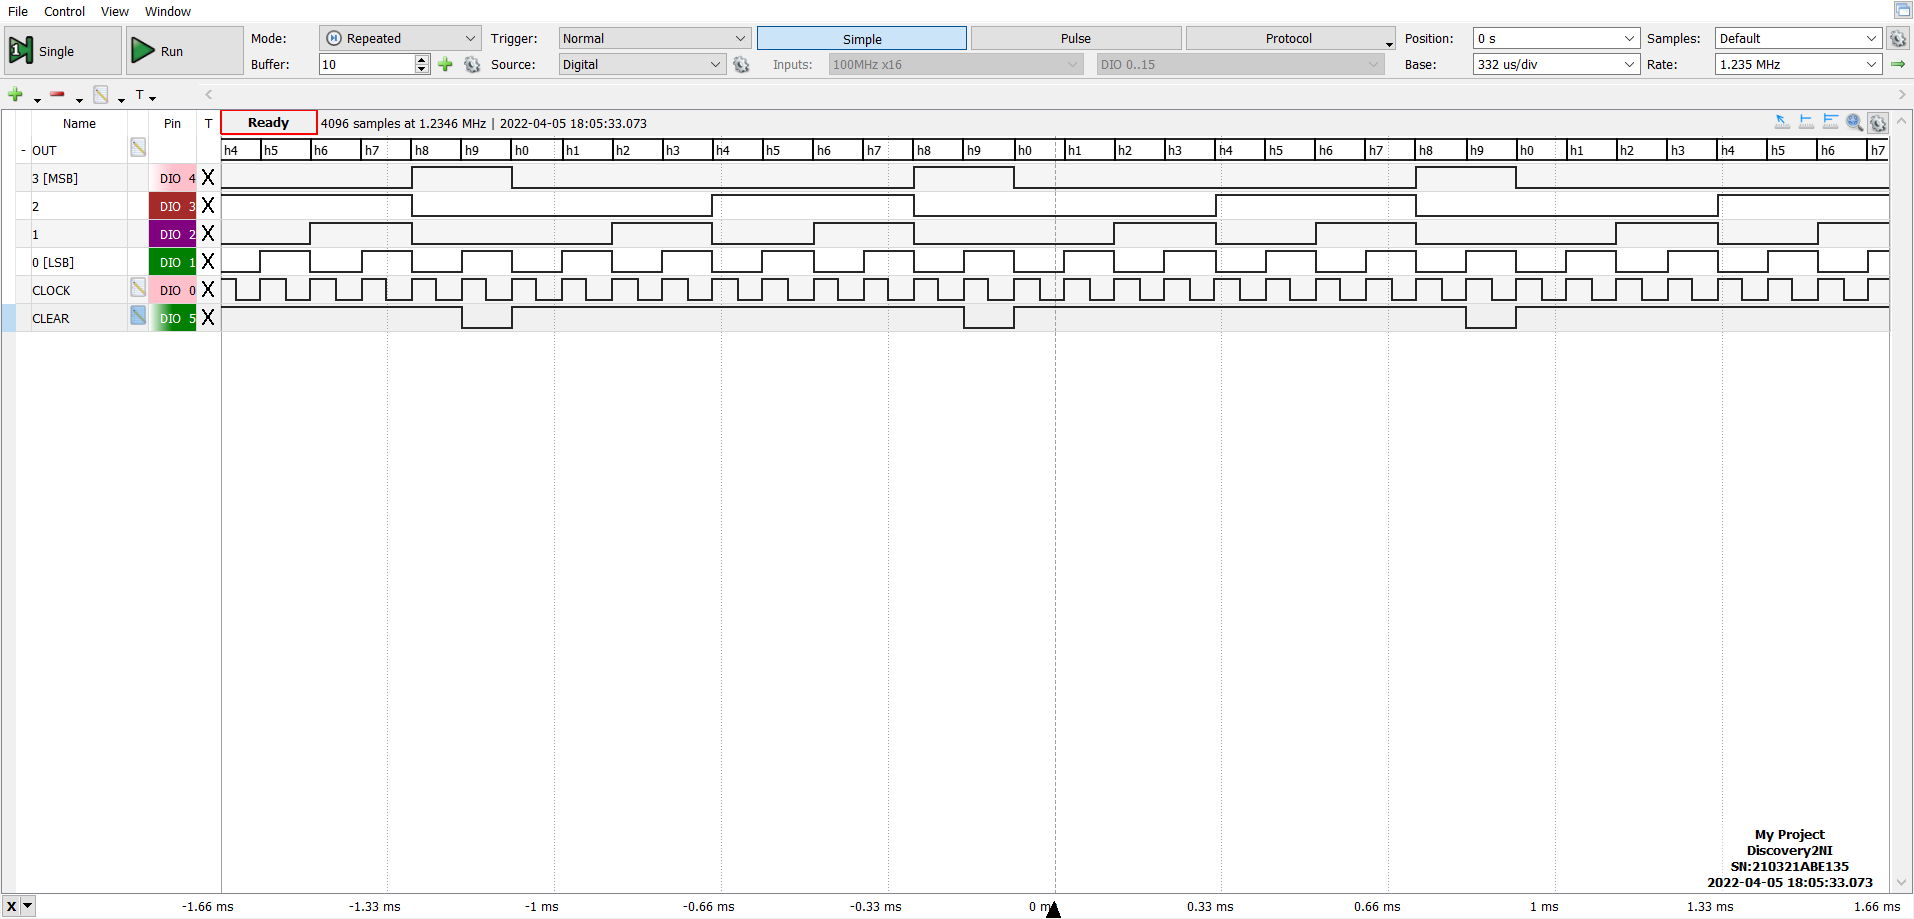
\includegraphics[width=\textwidth]{5.e}
	\caption{Acquisizione con Logic del bus in uscita dal circuito contatore BCD.
	Si può notare che il segnale presente in $Q_3$ ha periodo pari a 10 volte
	quello del clock \label{fig: Count_10th}}
\end{figure}

Come visibile dall'acquisizione riportata in \cref{fig: Count_10th}, troviamo
che il segnale in $Q_3$ è un'onda quadra di frequenza
$f = \nicefrac{f\ped{clk}}{10}$ come volevamo e Duty-Cycle pari al
$20 \percent$.

\subsection{Divisore di frequenza programmabile con RCO}
Infine si vuole costruire un divisore di frequenza programmabile:
per questo scopo utilizzeremo il bit RCO (Ripple Carry Output), la cui
funzione è di generare un segnale alto solo nel caso in cui il contatore abbia
raggiunto lo stato massimo $(1111)$ e il bit Load (Active-Low), che quando
è basso sovrascrive lo stato $Q_3, \ldots, Q_0$ del contatore con quello
presente nel bus di input $D_3, \ldots, D_0$. 
\begin{figure}[htbp]
\centering
	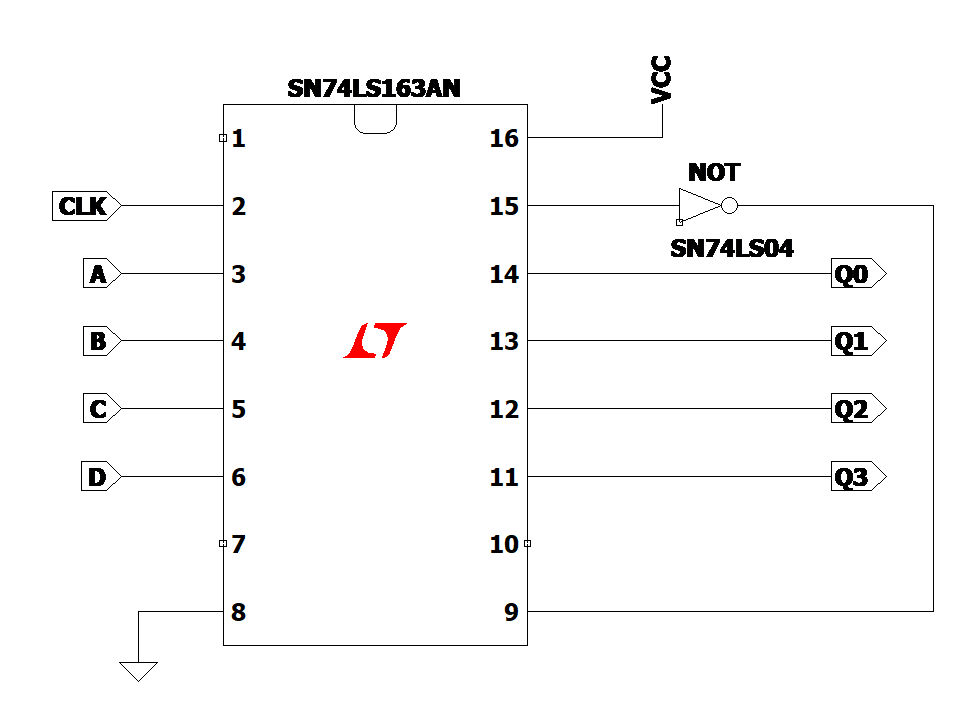
\includegraphics[width=0.6\textwidth]{Draft2}
	\caption{Schematica utilizzata per il divisore di frequenza programmabile
	\label{schem: programmable_counter}}
\end{figure}

Vogliamo preliminarmente verificare il funzionamento del RCO; dopo aver
montato nuovamento il circuito presente in \cref{fig: schem_counter} inviamo
un segnale di clock di frequenza 10 kHz e utilizziamo Logic per acquisire i
segnali del bus dei 4 bit di output e il segnale di RCO in funzione del tempo.
\begin{figure}[htbp]
\centering
	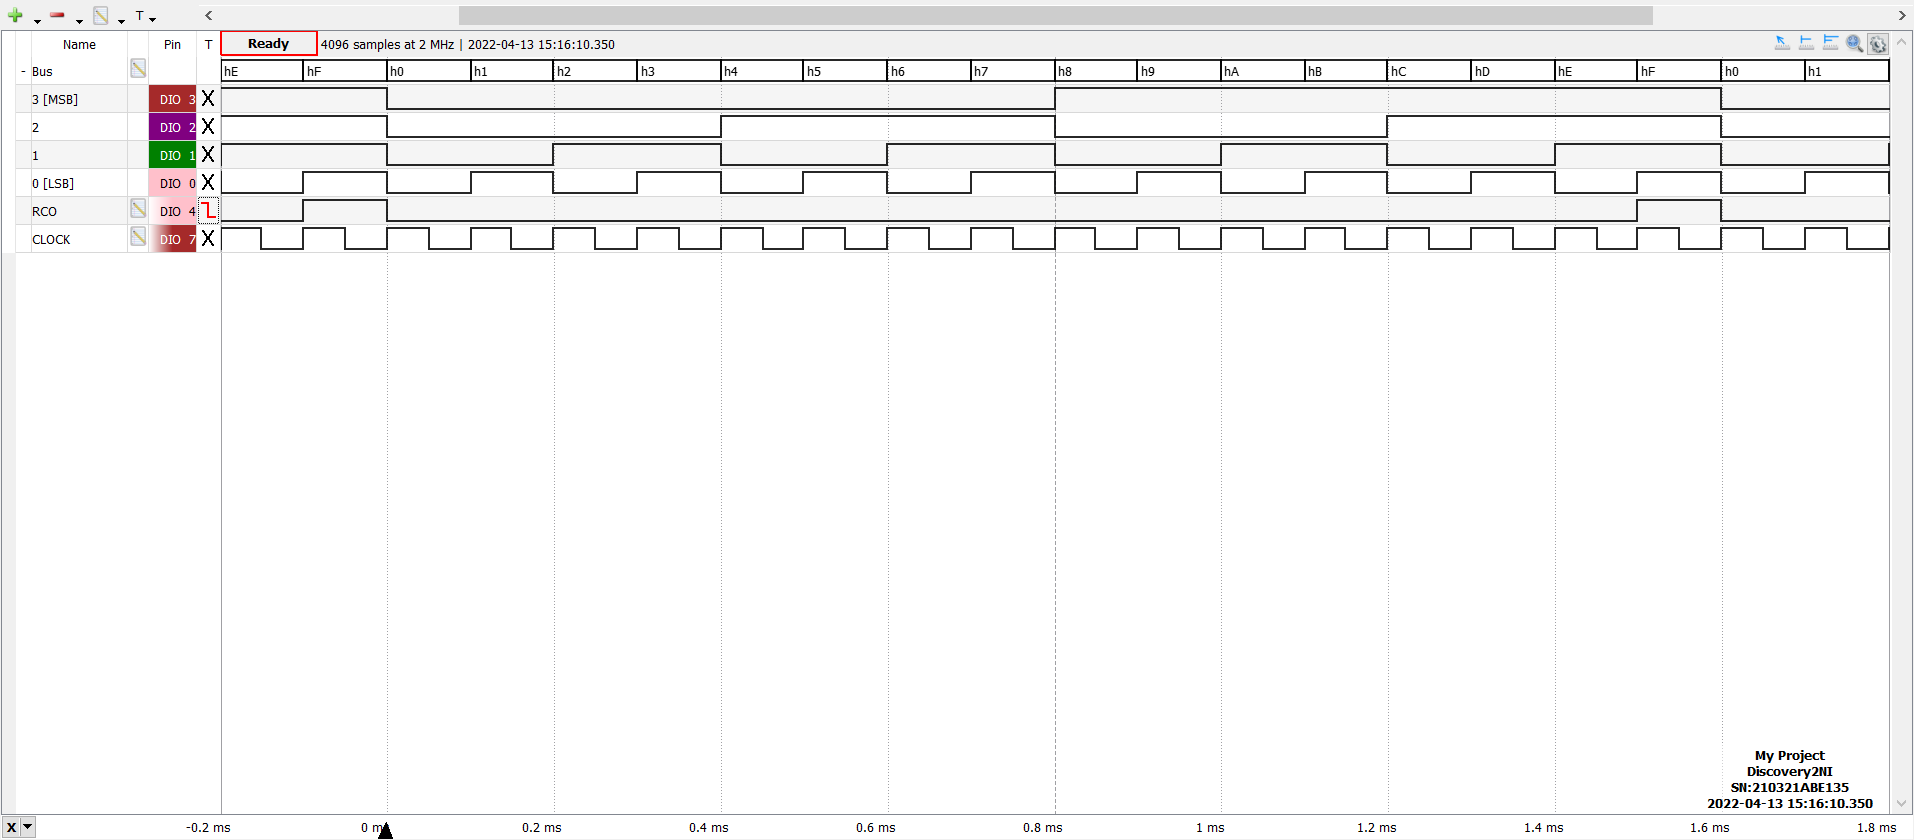
\includegraphics[width=\textwidth]{5.RCO}
	\label{fig: RCO_f}
	\caption{Acquisizione con Logic dei segnali in uscita dal contatore per
	verificare il funzionamento del bit RCO}
\end{figure}
Dall'acquisizione riportata in \cref{fig: RCO_f} possiamo notare che il bit
RCO funziona correttamente.

Quindi, per costruire il divisore programmabile schematizzato in
\cref{schem: programmable_counter} si collega l'uscita dal pin RCO all'ingresso
del pin LOAD dello stesso contatore tramite una porta NOT (integrato SN74LS04).
Si utilizza dunque la funzione StaticIO per caricare nel Bus di ingresso
lo stato $0101$ (5 arbitrariamente scelto), mantenendo collegato al circuito
il segnale di clock generato da Patterns. 
\begin{figure}[htbp]
\centering
	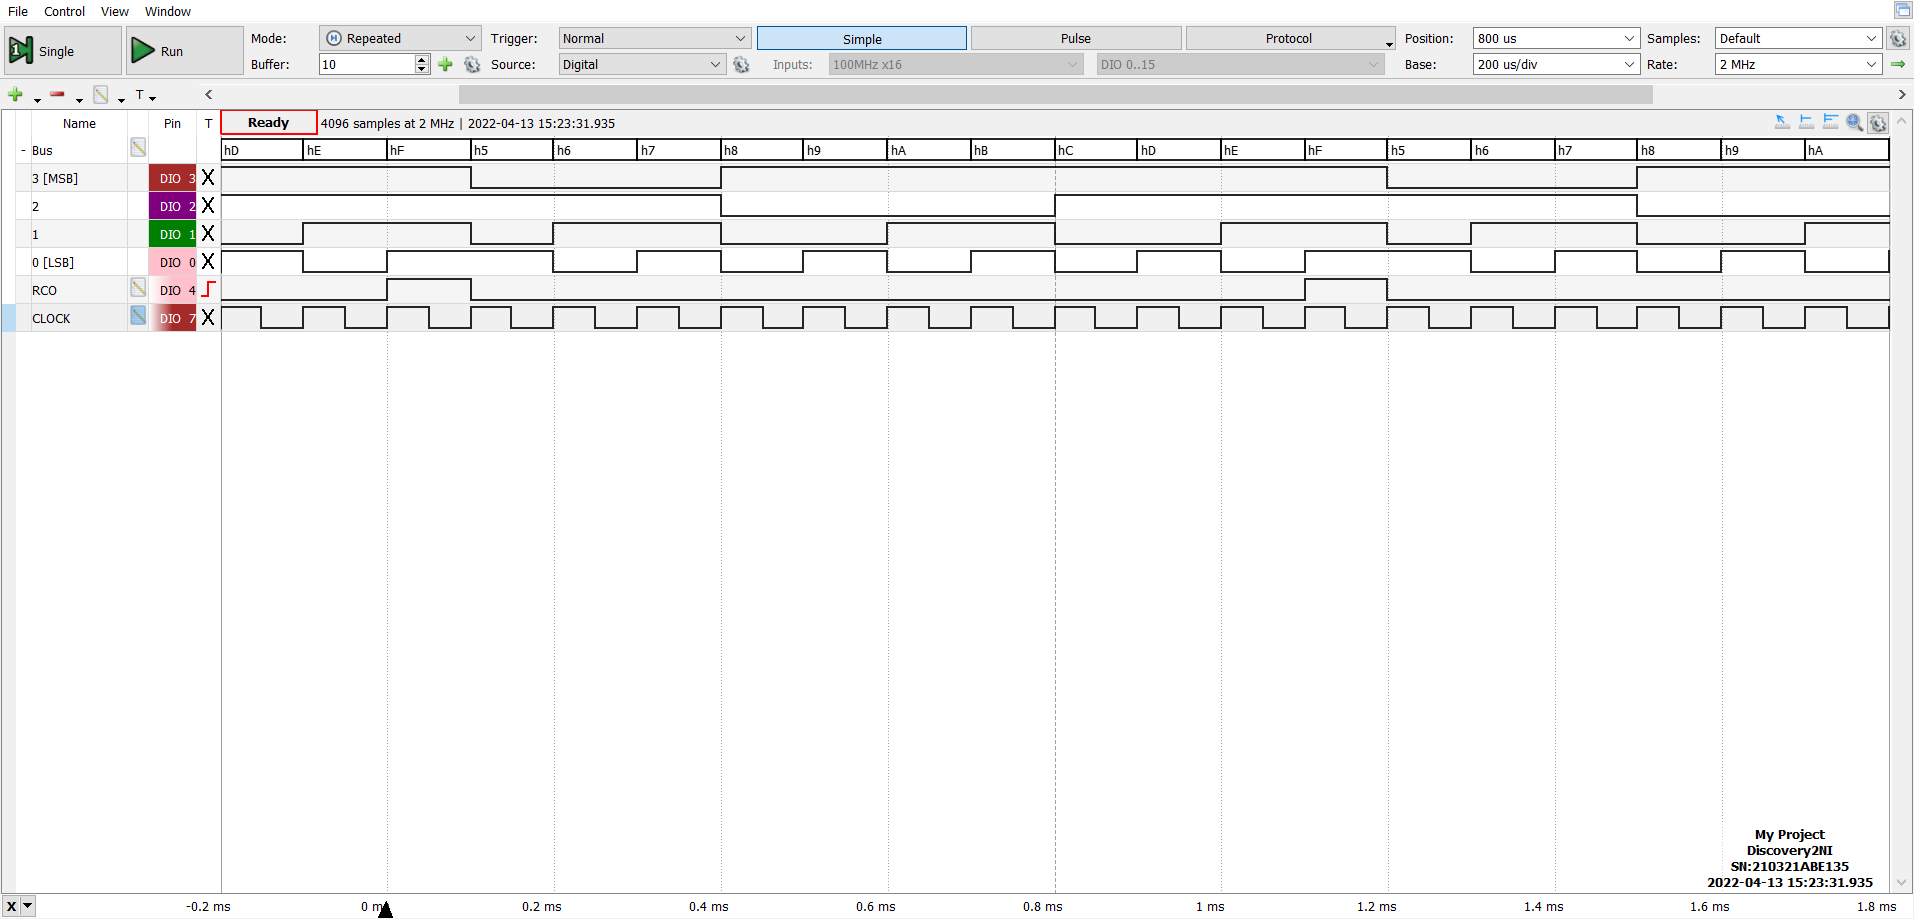
\includegraphics[width=\textwidth]{5.f_0101}
	\caption{Acquisizione con Logic dei segnali che interessano il circuito
	divisore di frequenza programmabile, con sequenza di avvio $0101$
	\label{fig: c_0101}}
\end{figure}
Dalla \cref{fig: c_0101} notiamo che quando il contatore riceve il
segnale di LOAD, quindi quando si registra 1 nel bit RCO, la sequenza iniziale
non viene immediatamente caricata, ma sarà posticipata da un evento di clock
($\approx 100 \; \si{\micro\s}$).
Di conseguenza, qualunque sia la sequenza iniziale del nostro circuito lo
stato finale 1111 verrà sempre "contato".

\subsection{Misura dei tempi caratteristici del divisore RCO}
Si cambia ora la sequenza di inizializzazione a $0110$, e utilizzando la
funzione Logic impostiamo un trigger quando il bit LOAD compie la transizione
$0 \to 1$: in seguito a quanto visto nella sezione precedente ci aspettiamo
che il contatore passi dallo stato $1111$ allo stato iniziale.

Visualizziamo i segnali sulle linee di dato e RCO su scala dei tempi molto
ristretta per misurare i ritardi tra di loro e verificare quanto affermato
nella \cref{sec: count_trans}.
\begin{figure}[htbp]
\centering
	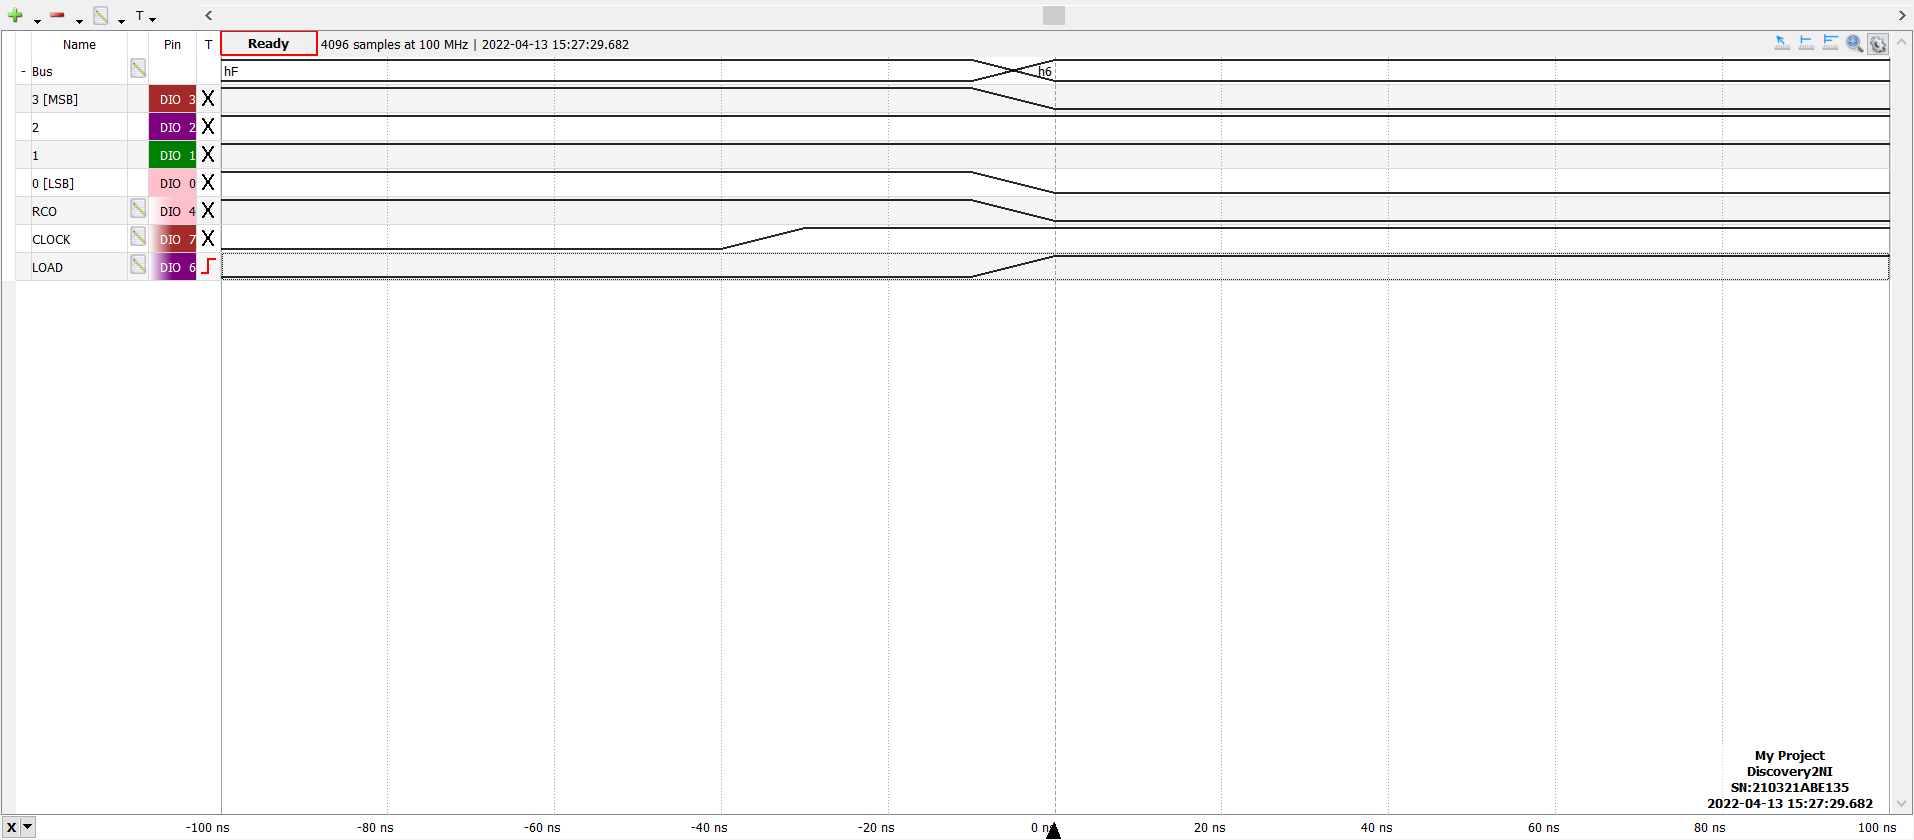
\includegraphics[width=\textwidth]{5.f_0110_20ns}
	\caption{Acquisizione con logic dei segnali di interesse per il circuito
	divisore di frequenza programmabile per un fondo scala dei tempi
	molto ristretto, con sequenza di avvio 0110
	\label{fig: count_20ns}}
\end{figure}
Dalla \cref{fig: count_20ns} si può notare che è sempre presente un ritardo
dall'inizio del nuovo fronte di salita del clock alla commutazione delle
uscite (che come prima è sincrona/simultanea) e che vale come prima
$30 \pm 10 \; \si{n\s}$, per cui la funzione di LOAD risulta sincrona.

\subsection{Analisi e verifica del comportamento del divisore RCO}
In questa sezione prendiamo la frequenza del segnale in uscita dal RCO come
frequenza quoziente/desiderata in uscita dal divisore.

Dato che RCO è attivo quando tutte le uscite $Q_i$ sono alte, il LOAD
(normalmente alto) viene attivato quando l'output corrisponde a 15. Al
fronte di salita del clock successivo le uscite vengono impostate ai valori
degli ingressi e il conteggio riparte. Dunque se si vuole realizzare un
divisore di frequenza $1/n$, o un contatore a $n$ stati, occorre impostare il
bus di input in modo che il conteggio parta da $16 - n$, quindi si osservano
in uscita i numeri da $(16 - n)_{16}$ fino a 15 ripetersi.

In altre parole ci si aspetta che il periodo del segnale RCO sia pari a
quello di clock moltiplicato per il numero di salti di stato necessari per
farlo arrivare a 0000; detto $I$ il valore (in base decimale) caricato nello
stato iniziale si ha dunque:
\begin{equation}
T\ped{divisore, I} = T\ped{clk} \cdot (16 - I)
\end{equation}
Visto però il funzionamento dei pin LOAD e RCO, se utilizzassimo come sequenza
iniziale 1111, il circuito produrrebbe un segnale costante: infatti 1111 è
anche lo stato a cui avviene il caricamento della sequenza, che però risulta
essere sempre la medesima, inducendo quindi uno stato incommutabile.

Programmando la sequenza iniziale a $0000$ invece ci si aspetta che il
comportamento del circuito si riduca allo stesso visto precedentemente in
\cref{sec: count_base} essendo 0000 lo stato iniziale a cui si resetta
autonomamente il counter in assenza di segnali di LOAD.

Si provano quindi diverse sequenze per inizializzare il contatore, per cui
in particolare ci si aspetta di trovare:
\begin{table}[htbp]
\centering
\begin{tabular}{c|c}
\toprule
Seq. iniziale & $T\ped{RCO} [T\ped{clk}]$\\
\midrule
$0000$ & $16$ \\
$0010$ & $14$ \\
$0101$ & $11$ \\
$1110$ & $2$ \\
$1111$ & $0$ \\
\bottomrule
\end{tabular}
\end{table}

\begin{figure}[htbp]
\centering
	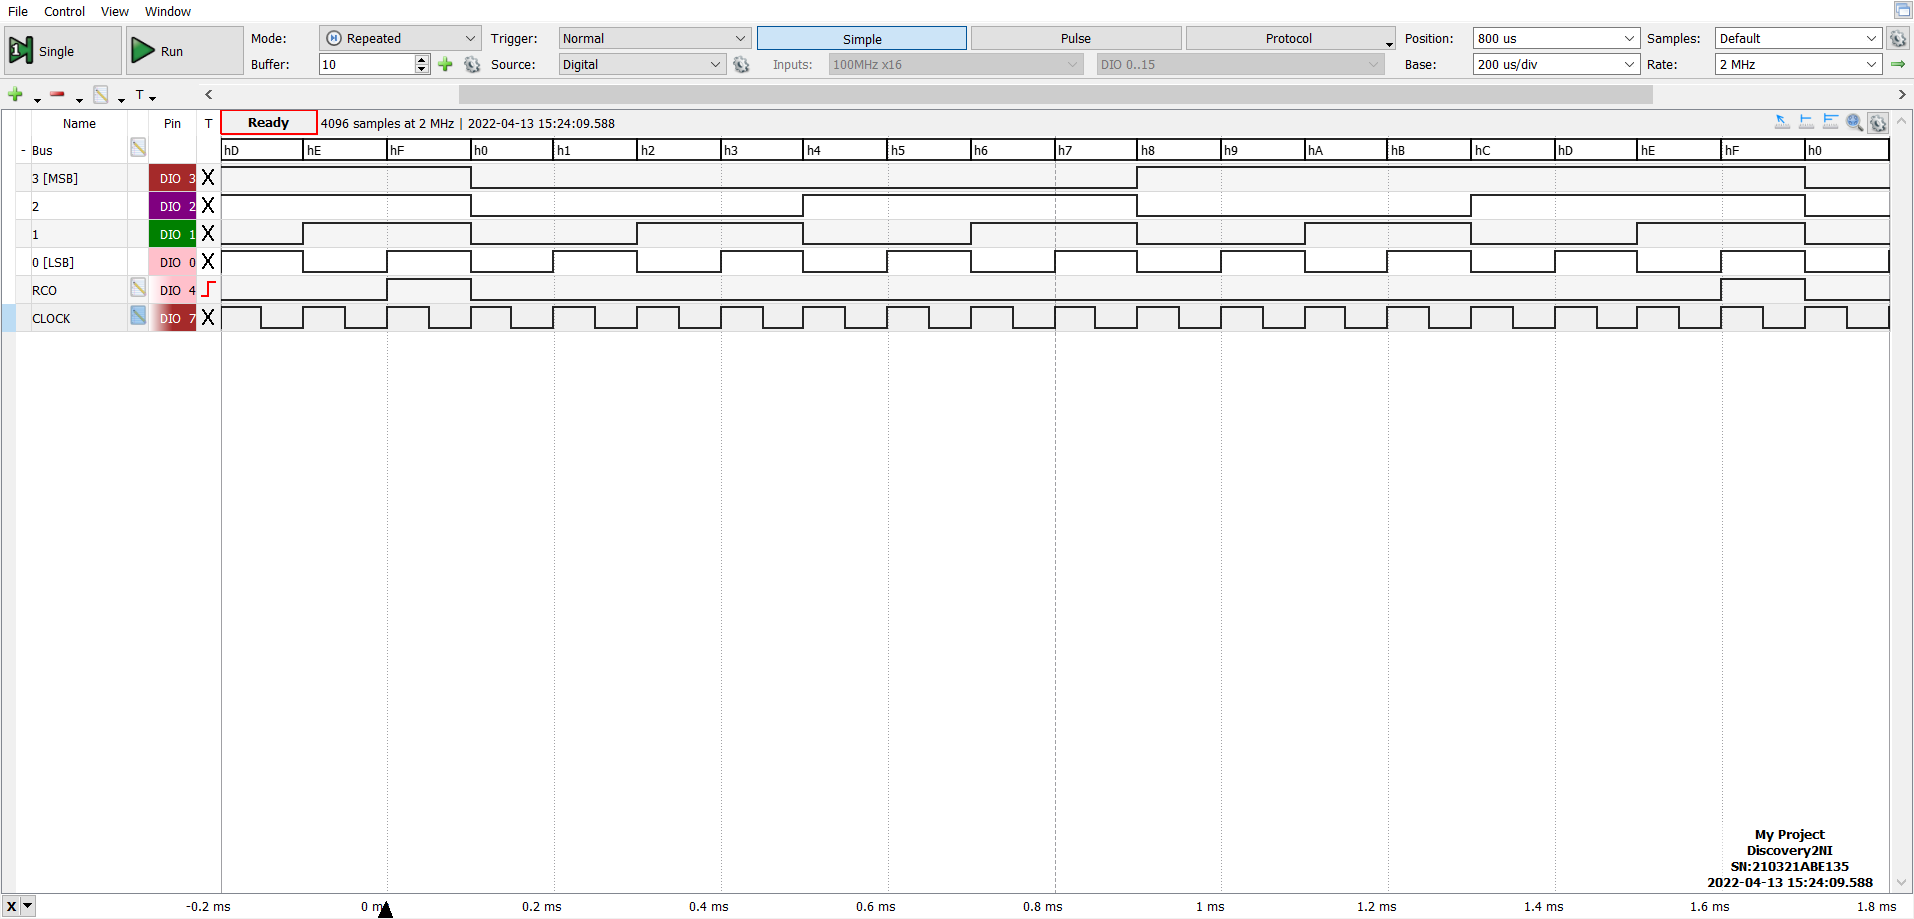
\includegraphics[width=\textwidth]{5.f_0000}
	\caption{Acquisizione con Logic dei segnali di interesse per il circuito divisore di frequenza programmabile, con sequenza di avvio 0000, da cui si misura $T = 16 T\ped{clk}$
	 \label{fig: RCO_0000}}
\end{figure}
\begin{figure}[htbp]
\centering
	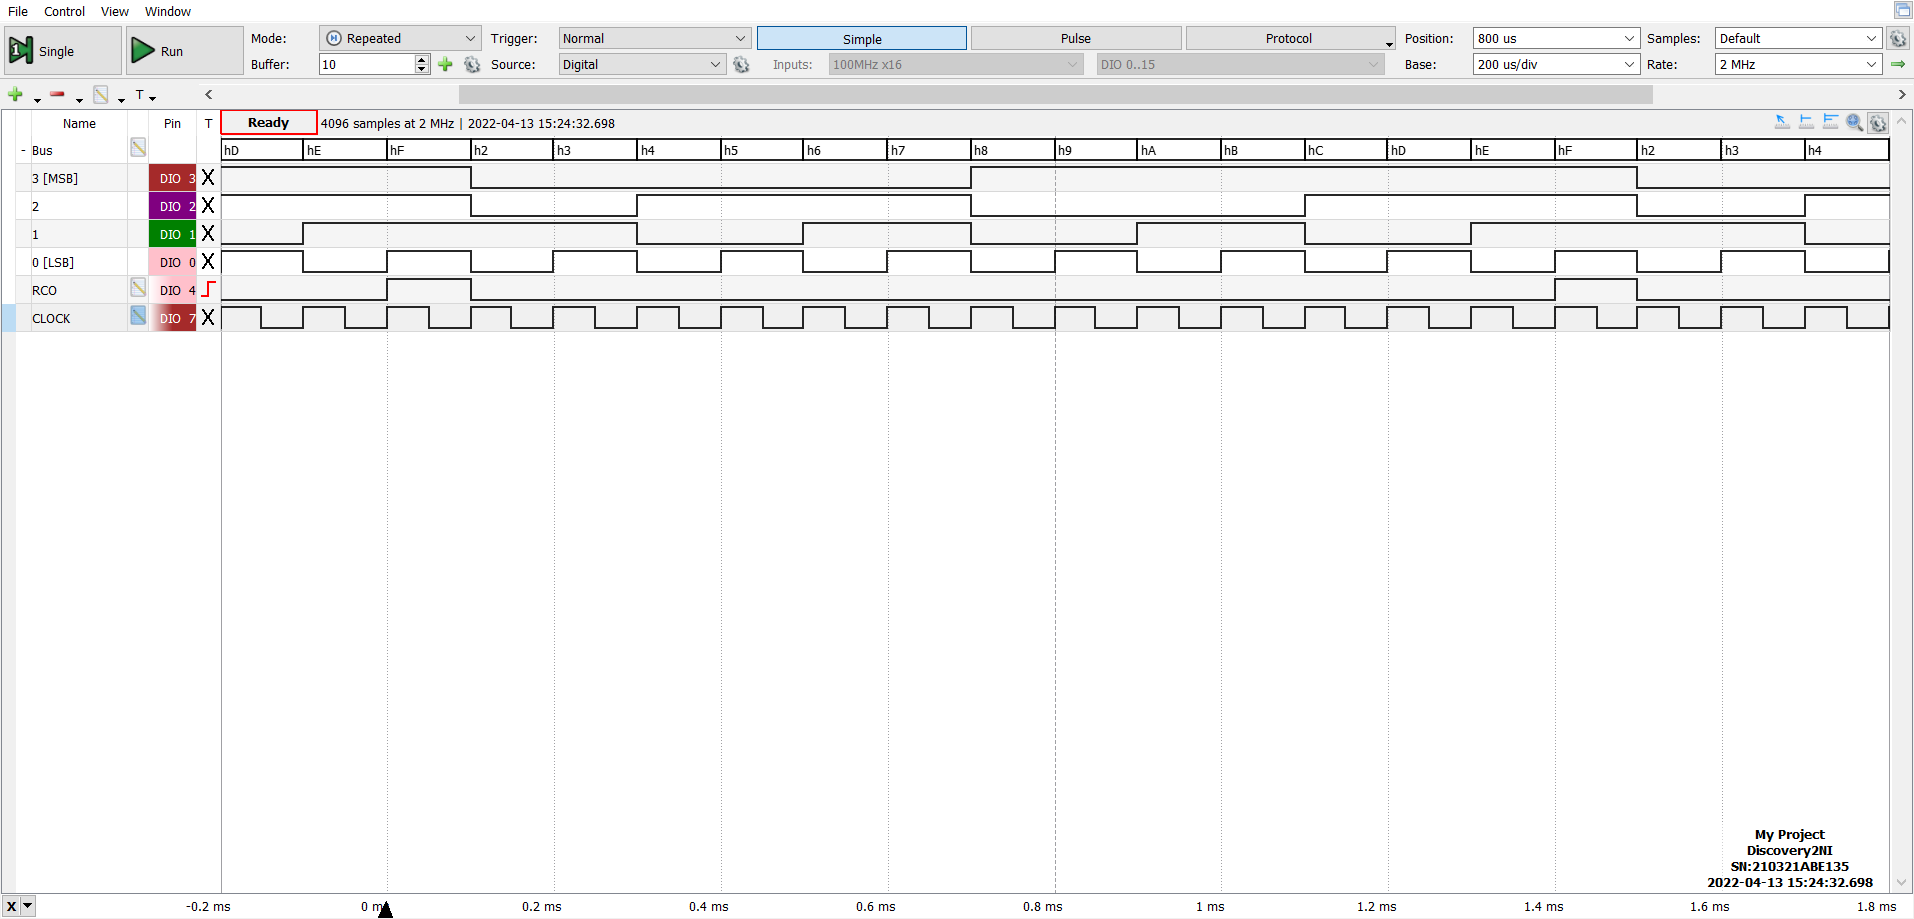
\includegraphics[width=\textwidth]{5.f_0010}
	\caption{Acquisizione con Logic dei segnali di interesse per il circuito divisore di frequenza programmabile, con sequenza di avvio 0010, da cui si misura $T = 14 T\ped{clk}$
	 \label{fig: RCO_0010}}
\end{figure}
\begin{figure}[htbp]
\centering
	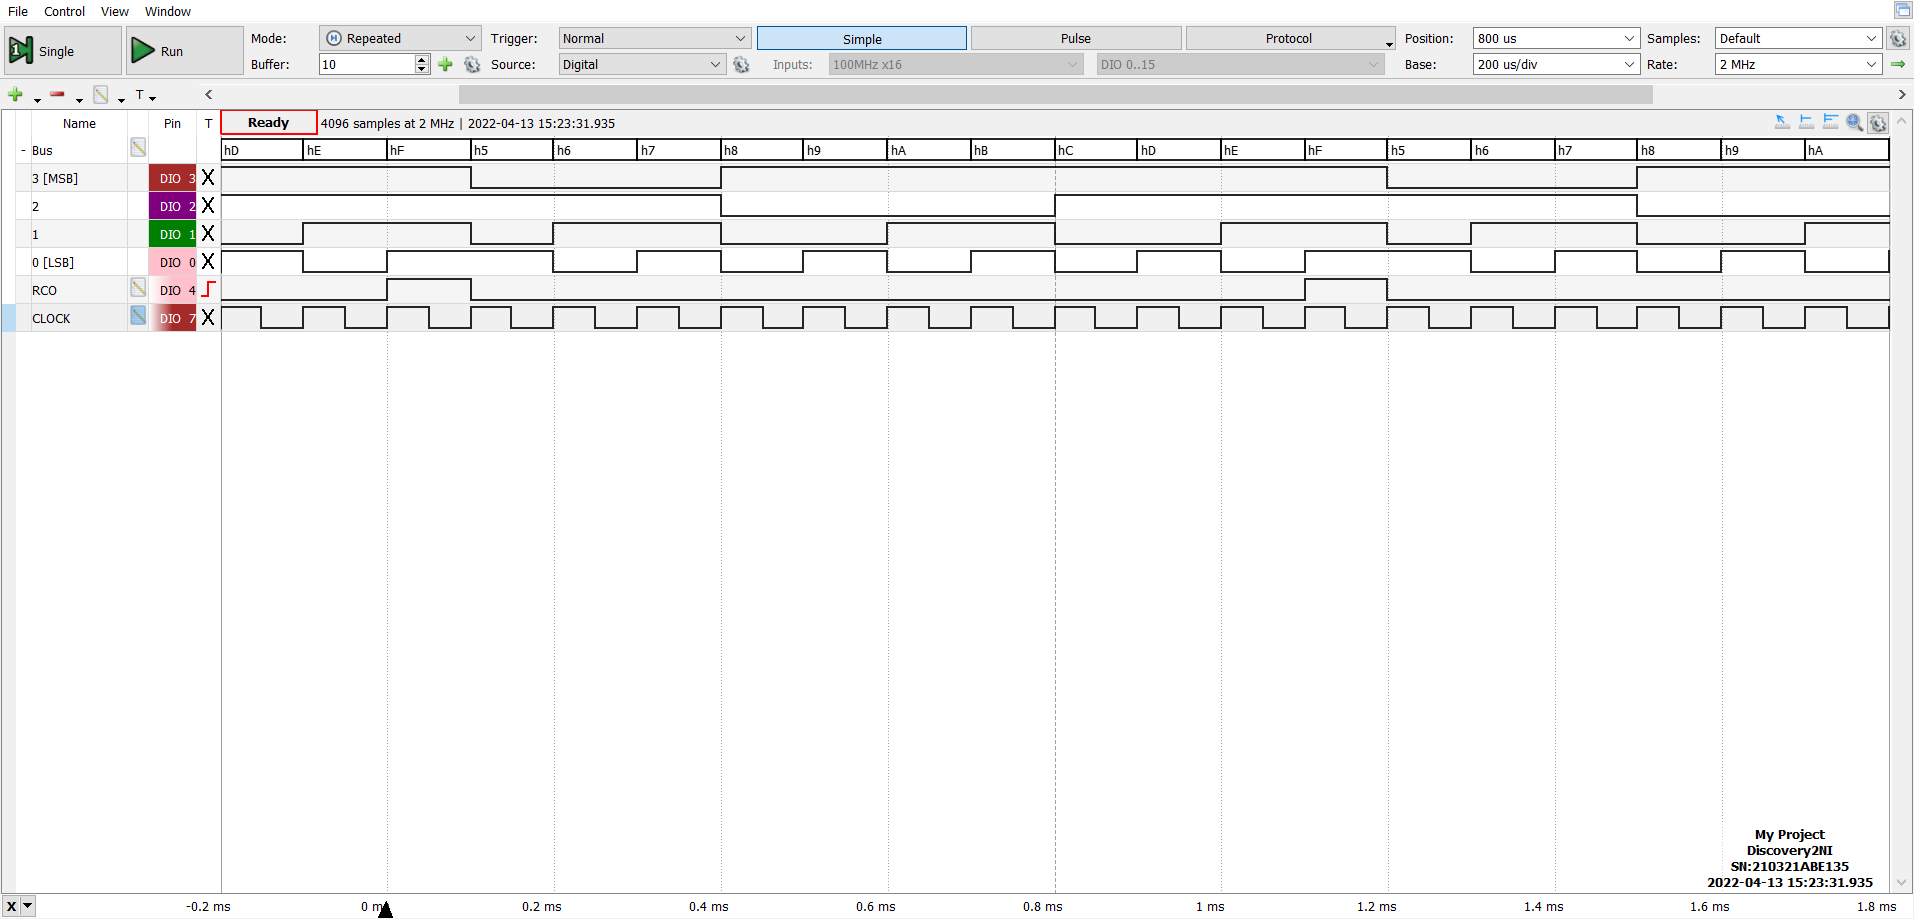
\includegraphics[width=\textwidth]{5.f_0101}
	\caption{Acquisizione con Logic dei segnali di interesse per il circuito divisore di frequenza programmabile, con sequenza di avvio 0101, da cui si misura $T = 11 T\ped{clk}$
	 \label{fig: RCO_0101}}
\end{figure}
\begin{figure}[htbp]
\centering
	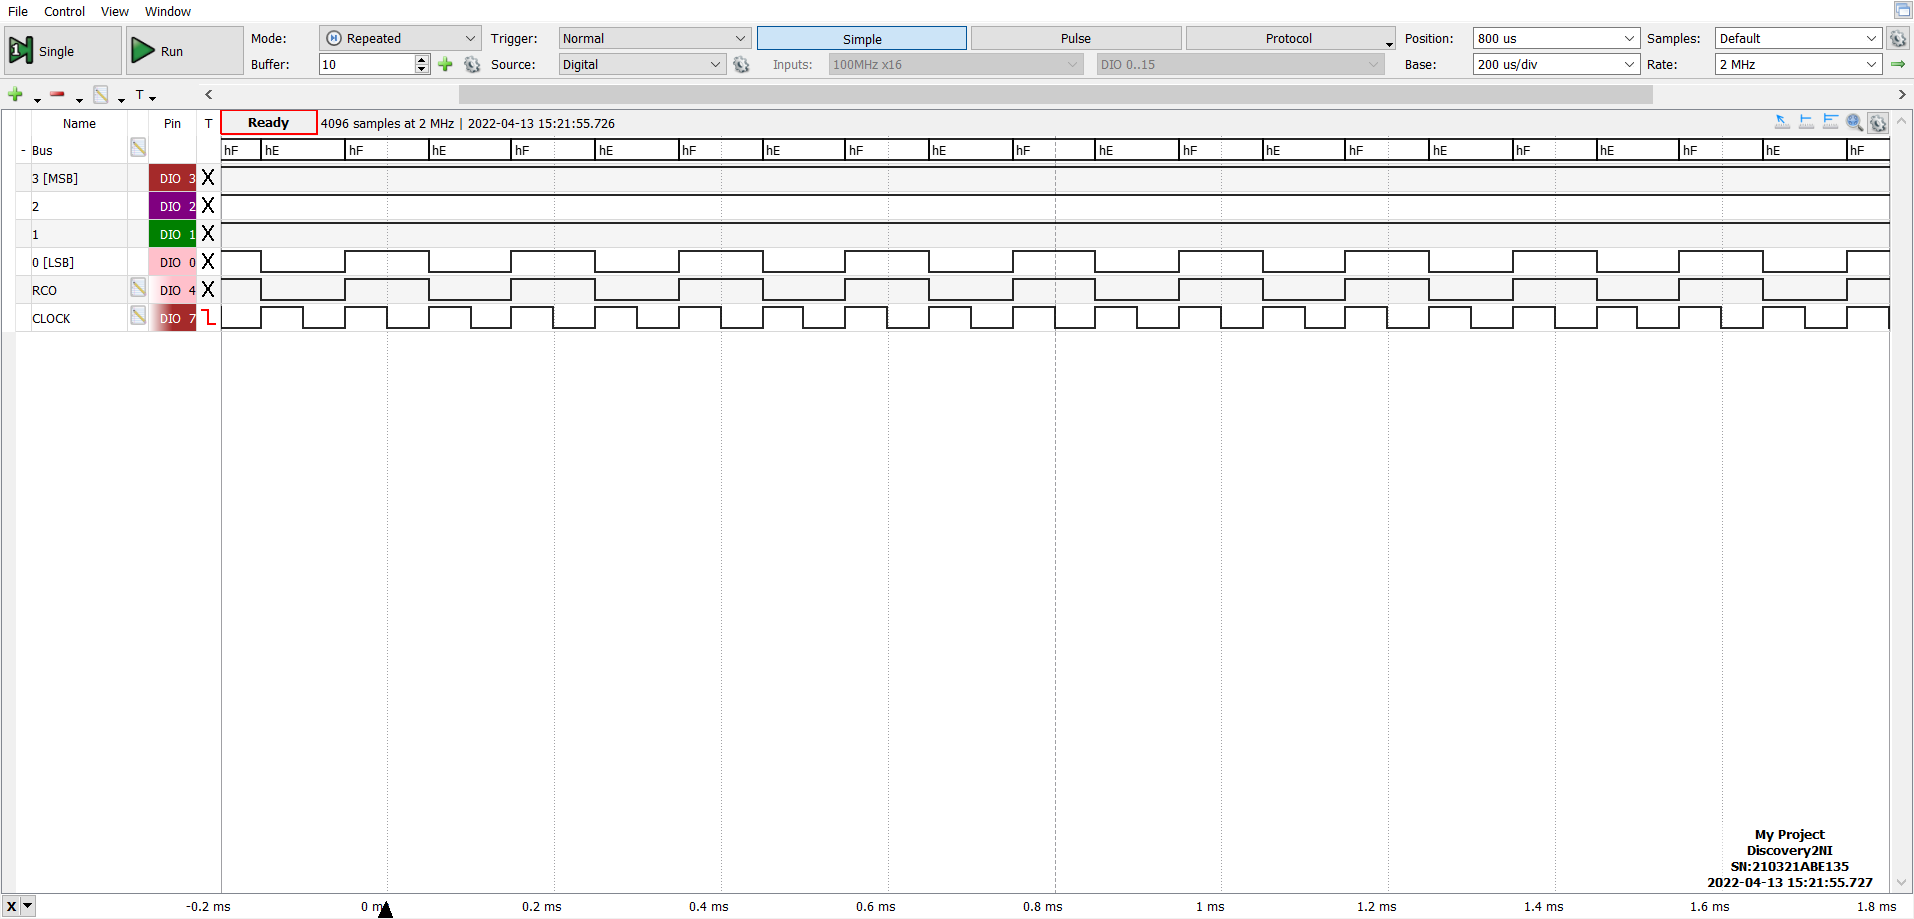
\includegraphics[width=\textwidth]{5.f_1110}
	\caption{Acquisizione con Logic dei segnali di interesse per il circuito divisore di frequenza programmabile, con sequenza di avvio 1110, da cui si misura $T = 2 T\ped{clk}$
	 \label{fig: RCO_1110}}
\end{figure}
\begin{figure}[htbp]
\centering
	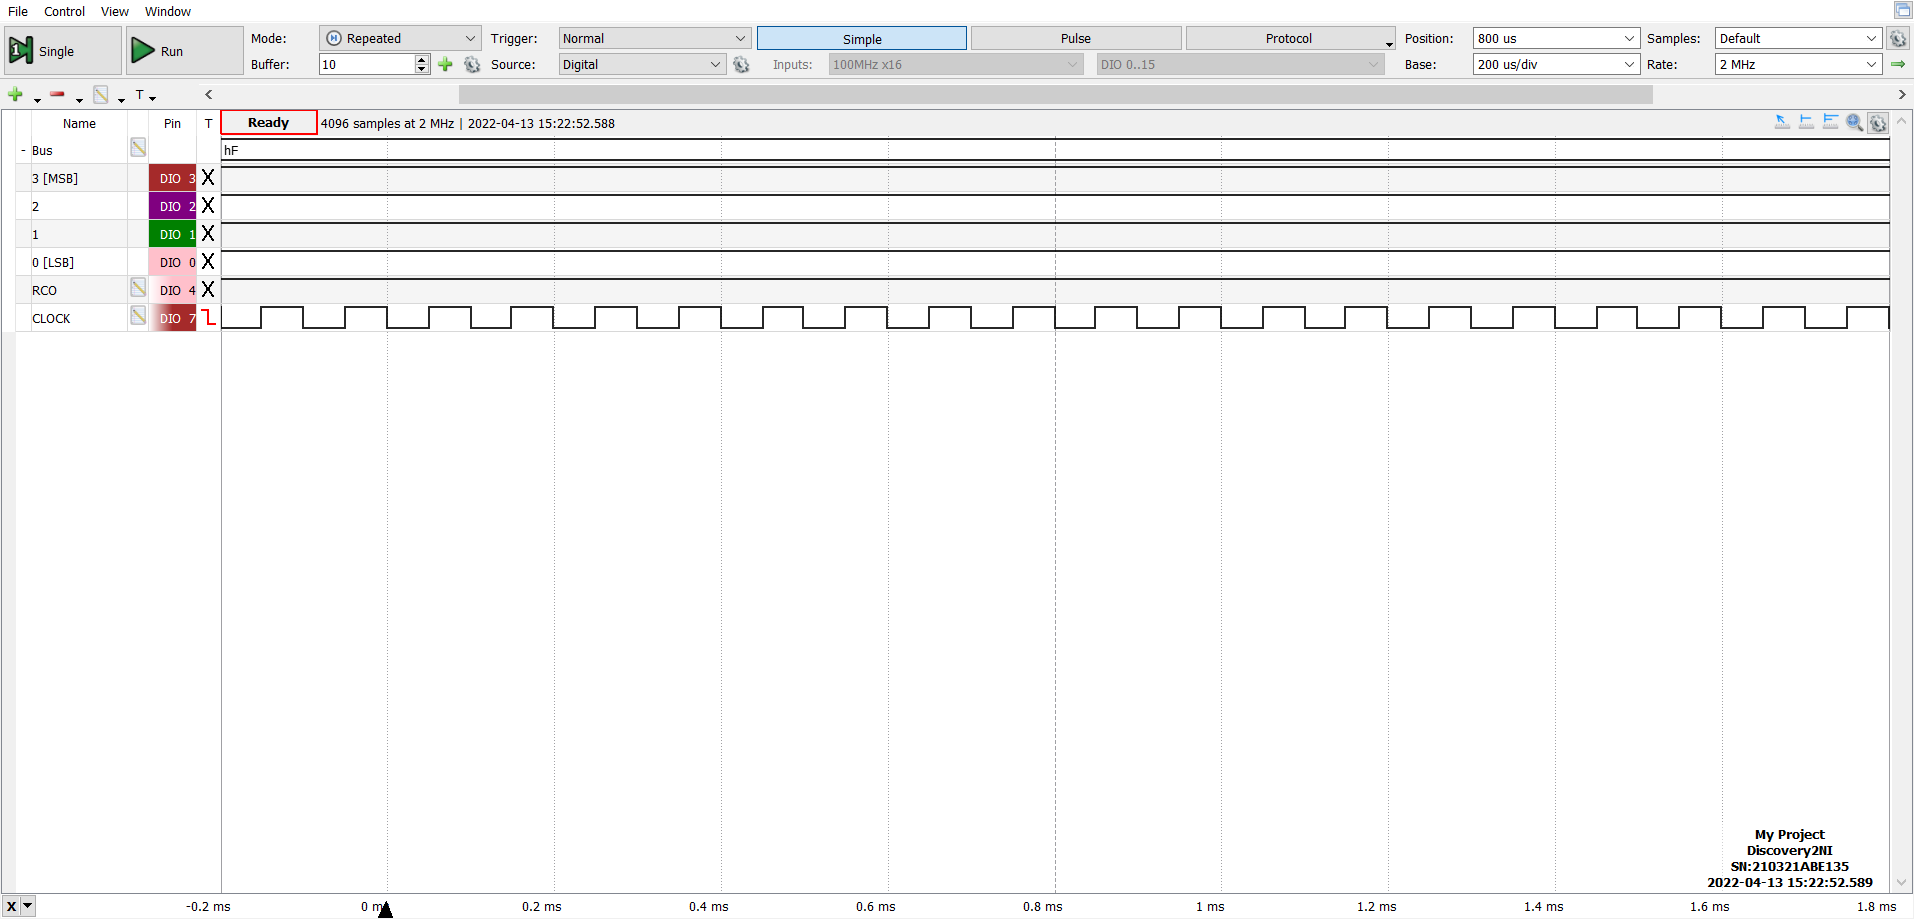
\includegraphics[width=\textwidth]{5.f_1111}
	\caption{Acquisizione con Logic dei segnali di interesse per il circuito divisore di frequenza programmabile, con sequenza di avvio 1111, dal quale si vede che RCO è un segnale costante \label{fig: RCO_1111}}
\end{figure}

Dalle acquisizioni del Logic Analyzer riportate in si vede che il comportamento
del circuito è coerente con quanto ci aspettavamo.

%=======================
\section*{Conclusioni e commenti finali}
Si è riusciti a verificare il corretto funzionamento di circuiti logici
sequenziali di crescente complessità e svariate applicazioni (e.g., sistemi di
controllo e misura) costruiti con porte NOT, NAND, XOR, D-Latch e contatori
sincroni.
In particolare sono stati realizzati e studiati un D-Latch, uno shift-register
con positive edge-triggered D-FF, un generatore di sequenze pseudocasuali e
alcuni tipi di divisore di frequenza con contatori binari.
Inoltre si è riusciti ad apprezzare l'effetto dei tempi di propagazione
delle porte sul loro comportamento, seppur in maniera limitata dalla bassa
risoluzione temporale dell'AD2.

%=======================
\section*{Dichiarazione}
I firmatari di questa relazione dichiarano che il contenuto della relazione \`e
originale, con misure effettuate dai membri del gruppo, e che tutti i firmatari
hanno contribuito alla elaborazione della relazione stessa.

\end{document}
